\chapter{Grafici di misure}
In fisica spesso è possibile verificare una formula facendo variare una delle grandezze contenute e osservando su un grafico come varia un'altra grandezza. A questo scopo si predispone una tabella coi dati e poi si realizza un grafico avendo come obiettivo una buona leggibilità. Elencheremo di seguito una procedura passo-passo, per realizzare dei buoni grafici elencando tutte le caratteristiche indispensabili. Nelle prossime sezioni, realizzeremo, prima un grafico a mano, poi con l'uso del foglio di calcolo.
\section{Un esempio di grafico realizzato a mano}

Supponiamo di aver misurato la capacità $C$ di un condensatore (unità di misura picofarad, pF)  in funzione della distanza tra le armature di un condensatore piano (distanza d espressa in mm). I dati sono in tabella \ref{tab:condensatore}: 

\begin{table}
\begin{center}
{
\def\arraystretch{1.5} %serve a inserire spazio bianco
\begin{tabular}{|c|c|}
\hline 
 $d\left( \si{\milli\meter}\right)$ & $C \left( \si{\pico\farad}\right)$   \\
\hline
2 & 420\\
3 &  282 \\
4 &  219 \\
5 & 182 \\
6 & 158 \\
7 &  139\\
8 &  127\\
9  & 115\\
10 & 108\\
\hline
\end{tabular}
}
\caption{Dati per il grafico capacità-distanza}
\label{tab:condensatore}
\end{center}
\end{table}
La prima cosa che notiamo, è che all'aumentare della distanza, la capacità diminuisce. Questo tipo di andamento, vedremo, è indizio (ma non è sufficiente) di una proporzionalità inversa. Ti invito a realizzare il grafico che stiamo costruendo, anche col foglio di calcolo, usando il metodo che vedremo più avanti. Vediamo quali scelte vanno fatte per il grafico.
\subsection{Disegno degli assi e titolo del grafico}
Possiamo disegnare subito gli assi lungo il bordo arancione e dare un titolo al grafico (figura \ref{fig:titoloassi})

   \begin{figure}[h!]
    \centering
    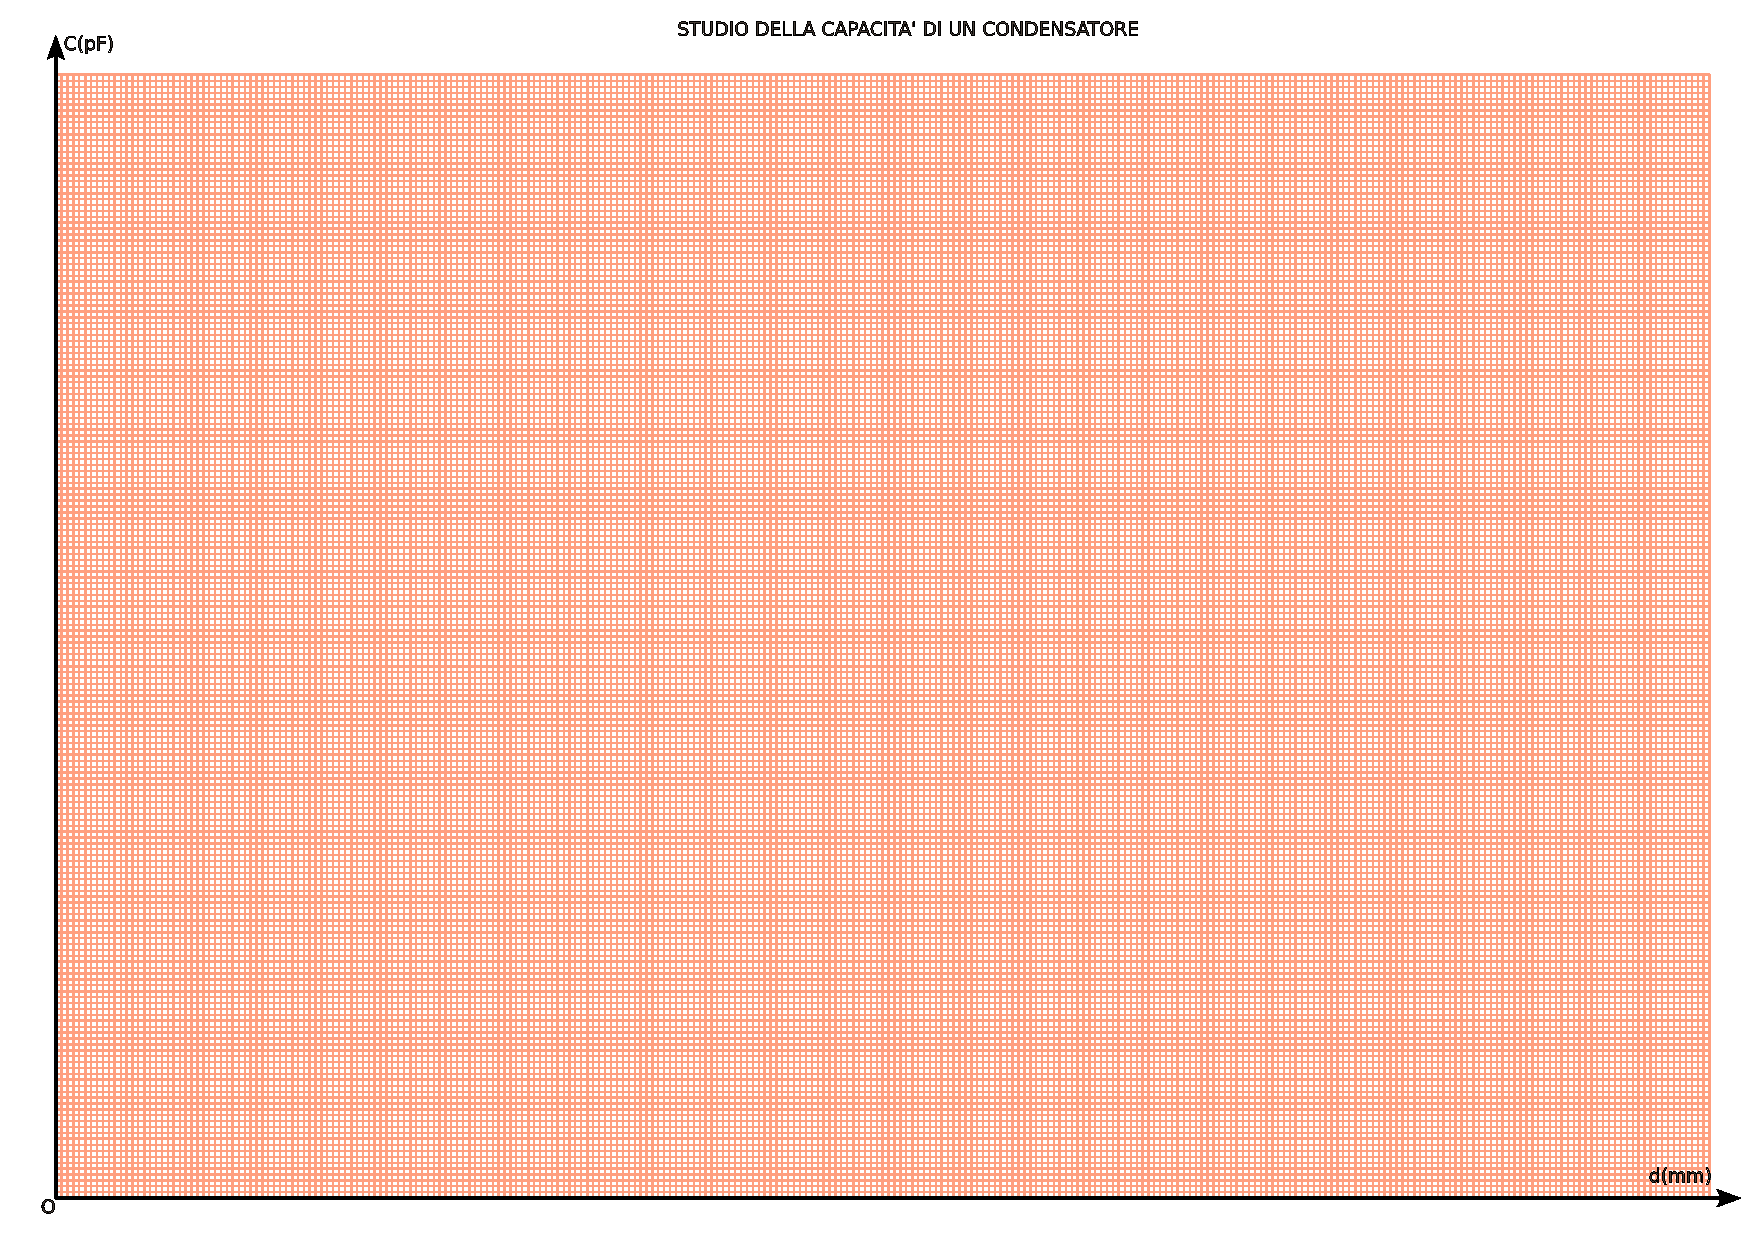
\includegraphics[width=\linewidth]{img/titoloassi.pdf} 
    \caption{Titolo e  etichette sugli assi}
    \label{fig:titoloassi}
\end{figure}  

\subsection{Scelta dei fattori di scala i valori maggiori} 
Per scegliere la scala, dobbiamo calcolare approssimativamente dove vogliamo che il grafico termini, e poiché vogliamo che venga grande, faremo in modo che i valori massimi delle due variabili capitino alla fine del foglio. Abbiamo un foglio in cui l'area arancione ha   dimensioni di $280 \times 200 $ millimetri e vogliamo che il massimo valore della distanza in tabella, ossia $\SI{10}{\milli\meter}$, capiti alla fine dell'asse X ad una distanza di circa $\SI{280}{\milli\meter}$. Dunque calcoliamo il fattore di scala sull'asse X:
\[
F_x=\frac{\SI{280}{\milli\meter}}{\SI{10}{\milli\meter}} = 28
\]
Con questo fattore potremo inserire ogni dato della prima colonna sul grafico moltiplicandolo per $F_x$. Per esempio, il valore $\SI{2}{\milli\meter}$ andrà inserito sul punto dell'asse X di ascissa $28\times\SI{2}{\milli\meter} = \SI{56}{\milli\meter}$. Analogamente, il fattore di scala sull'asse Y è:
\[
F_y = \frac{\SI{200}{\milli\meter}}{\SI{420}{\pico\farad}} = \SI{0,476}{\milli\meter\per\pico\farad}.
\] 

E' sempre meglio approssimare per difetto i fattori di scala, altrimenti i valori massimi della tabella, potrebbero uscire dai bordi del foglio (dalla parte colorata).
Effettuando i calcoli, otteniamo per i dati sull'asse X:
\begin{equation*}
\begin{aligned}
\SI{2}{\milli\meter} \times 28 &= \SI{56}{\milli\meter}  \\
\SI{3}{\milli\meter}  \times 28 &= \SI{84}{\milli\meter}  \\
\SI{4}{\milli\meter}  \times 28 &= \SI{112}{\milli\meter}   \\
\SI{5}{\milli\meter}  \times 28 &= \SI{140}{\milli\meter}  \\
\SI{6}{\milli\meter}  \times 28 &= \SI{168}{\milli\meter}   \\
\SI{7}{\milli\meter}  \times 28 &= \SI{196}{\milli\meter}  \\
\SI{8}{\milli\meter}  \times 28 &= \SI{224}{\milli\meter}  \\
\SI{9}{\milli\meter}  \times 28 &= \SI{252}{\milli\meter}  \\
\SI{10}{\milli\meter}  \times 28 &= \SI{280}{\milli\meter}  \\
\end{aligned}
\end{equation*}
Facciamo anche i calcoli per i dati da inserire sull'asse Y:

\[
\begin{array}{rcl}
\SI{420}{\pico\farad} \times \SI{0.476}{\milli\meter\per\pico\farad} &=& \SI{199.92}{\milli\meter} \\
\SI{282}{\pico\farad} \times \SI{0.476}{\milli\meter\per\pico\farad} &=& \SI{134.232}{\milli\meter} \\
\SI{219}{\pico\farad} \times \SI{0.476}{\milli\meter\per\pico\farad} &=& \SI{104.244}{\milli\meter} \\
\SI{182}{\pico\farad} \times \SI{0.476}{\milli\meter\per\pico\farad} &=& \SI{86.632}{\milli\meter} \\
\SI{158}{\pico\farad} \times \SI{0.476}{\milli\meter\per\pico\farad} &=& \SI{75.208}{\milli\meter} \\
\SI{139}{\pico\farad} \times \SI{0.476}{\milli\meter\per\pico\farad} &=& \SI{66.164}{\milli\meter} \\
\SI{127}{\pico\farad} \times \SI{0.476}{\milli\meter\per\pico\farad} &=& \SI{60.452}{\milli\meter} \\
\SI{115}{\pico\farad} \times \SI{0.476}{\milli\meter\per\pico\farad} &=& \SI{54.74}{\milli\meter} \\
\SI{108}{\pico\farad} \times \SI{0.476}{\milli\meter\per\pico\farad} &=& \SI{51.408}{\milli\meter} \\
\end{array}
\]
Ovviamente, questi valori devono essere arrotondati per difetto al millimetrio più vicino (il foglio permette al massimo di tracciare i millimetri). Queste due tabelle dei calcoli, non vanno riportate sul foglio di relazione ma solo sui propri appunti. Quello che ci interessa sono i numeri finali (i millimetri). Riportiamo in fine, i dati sul grafico (figura \ref{fig:graficomanuale}) dove abbiamo anche tracciato (ad occhio) una linea di tendenza. 
 
    \begin{figure}[h!]
    \centering
    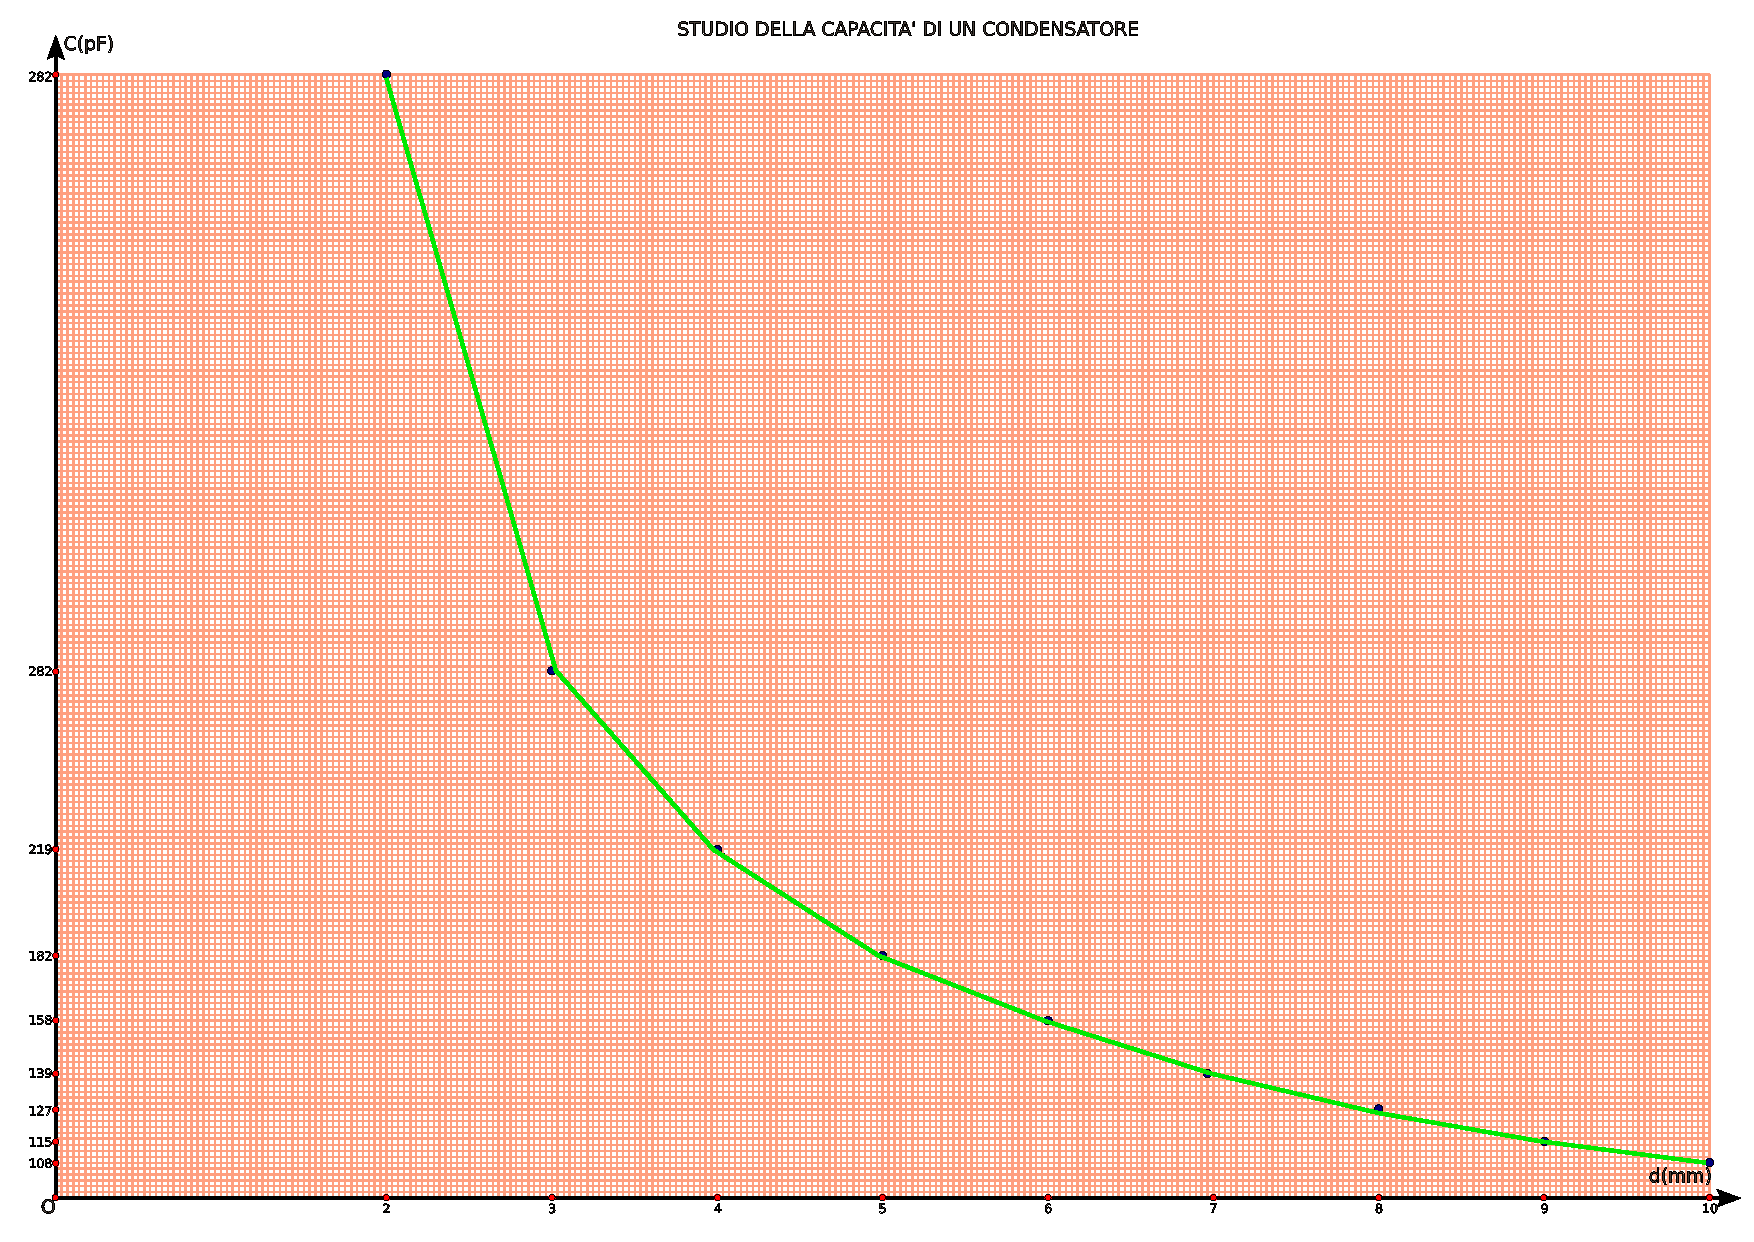
\includegraphics[width=\linewidth]{img/graficomanuale.pdf} 
    \caption{Grafico su carta millimetrata.}
    \label{fig:graficomanuale}
\end{figure}


\section{Rette di massima e minima pendenza}\label{sec:rettemaxmin}
Quando i dati sperimentali si dispongono lungo una retta, spesso lo scopo dell'esperimento è misurare la \textbf{pendenza} di quella retta, perché la pendenza ha un significato fisico (una velocità, una costante elastica, l'accelerazione di gravità\dots). Tracciando ``a occhio'' una sola linea di tendenza otteniamo un valore per la pendenza, ma non la sua incertezza. Il \textbf{metodo delle rette di massima e minima pendenza} serve proprio a stimare l'errore sulla pendenza a partire dalle barre d'errore dei dati.

\subsection{I quattro punti di ancoraggio}
Si considerano solo il \textbf{primo} punto sperimentale $P_1(x_1,y_1)$ e l'\textbf{ultimo} $P_n(x_n,y_n)$, cioè quelli agli estremi del grafico, e le loro barre d'errore verticali di semiampiezza $e_y$ (l'incertezza sulla grandezza in ordinata). Sugli estremi delle due barre individuiamo quattro punti:
\begin{itemize}
\item sulla barra di $P_1$: \; $A=(x_1,\; y_1+e_y)$ \; (estremo superiore) \quad e \quad $B=(x_1,\; y_1-e_y)$ \; (estremo inferiore);
\item sulla barra di $P_n$: \; $C=(x_n,\; y_n+e_y)$ \; (estremo superiore) \quad e \quad $D=(x_n,\; y_n-e_y)$ \; (estremo inferiore).
\end{itemize}

\subsection{Costruzione delle due rette}
\begin{itemize}
\item la \textbf{retta di massima pendenza} congiunge $B$ (in basso a sinistra) con $C$ (in alto a destra): è la retta più ``ripida'' compatibile con le barre d'errore;
\item la \textbf{retta di minima pendenza} congiunge $A$ (in alto a sinistra) con $D$ (in basso a destra): è la retta meno ``ripida''.
\end{itemize}
Le due pendenze si calcolano con la solita formula $m=\dfrac{y_{\text{fin}}-y_{\text{in}}}{x_{\text{fin}}-x_{\text{in}}}$:
\[
m_{max}=\frac{(y_n+e_y)-(y_1-e_y)}{x_n-x_1}, \qquad
m_{min}=\frac{(y_n-e_y)-(y_1+e_y)}{x_n-x_1}.
\]
Il valore da assumere per la pendenza e la sua incertezza si ottengono poi come valore medio e semidispersione:
\[
\colorboxed{ocre}{m=\frac{m_{max}+m_{min}}{2}}, \qquad
\colorboxed{ocre}{\Delta m=\frac{m_{max}-m_{min}}{2}}.
\]
Un controllo va sempre fatto: entrambe le rette limite devono passare (o quasi) anche \emph{attraverso le barre d'errore dei punti intermedi}. Se così non è, o i dati non sono davvero lineari, oppure alcune barre d'errore sono state sottostimate.

\subsection{Esempio: la legge di Hooke}
Misurando l'allungamento $\Delta x$ di una molla al variare della forza applicata $F$, ci si aspetta la relazione lineare $F=k\,\Delta x$, dove $k$ è la costante elastica (pendenza della retta). I dati sono in tabella \ref{tab:hooke}; l'incertezza sulla forza è $e_F=\SI{0,10}{\newton}$, quella sull'allungamento è trascurabile.

\begin{table}[h!]
\centering
\begin{tabular}{ccccc}
\toprule
 & $P_1$ & $P_2$ & $P_3$ & $P_4$ \\
\midrule
$\Delta x$ (m) & 0,010 & 0,021 & 0,032 & 0,041 \\
$F$ (N)        & 0,49  & 0,98  & 1,47  & 1,96  \\
\bottomrule
\end{tabular}
\caption{Forza applicata e allungamento di una molla ($e_F=\SI{0,10}{\newton}$).}
\label{tab:hooke}
\end{table}

I quattro punti di ancoraggio sul primo e sull'ultimo dato sono:
\[
\begin{aligned}
A &= (0,010;\ 0,49+0,10) = (0,010;\ 0,59), & B &= (0,010;\ 0,49-0,10) = (0,010;\ 0,39),\\
C &= (0,041;\ 1,96+0,10) = (0,041;\ 2,06), & D &= (0,041;\ 1,96-0,10) = (0,041;\ 1,86).
\end{aligned}
\]

\begin{figure}[h!]
\centering
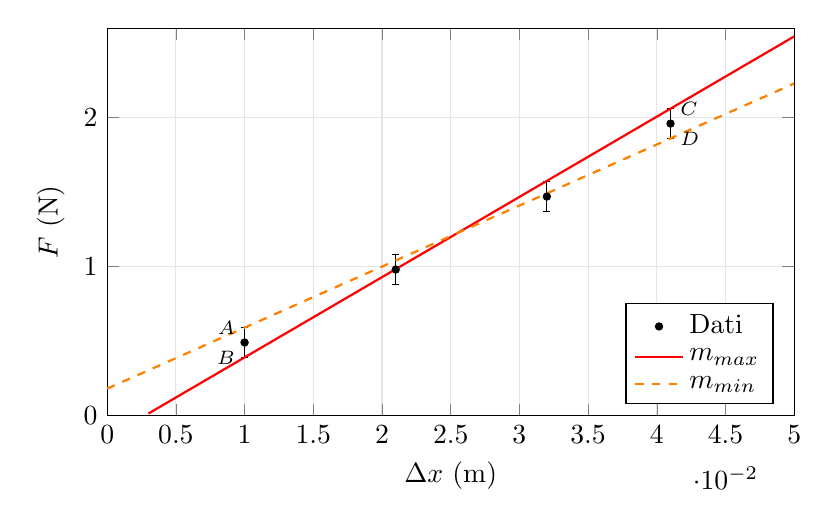
\begin{tikzpicture}
\begin{axis}[
    width=0.85\linewidth, height=6.5cm,
    xlabel={$\Delta x$ (m)}, ylabel={$F$ (N)},
    xmin=0, xmax=0.05, ymin=0, ymax=2.6,
    legend pos=south east, legend cell align=left,
    grid=both, grid style={gray!20},
]
% dati con barra d'errore su F
\addplot[only marks, mark=*, mark size=1.3pt, black,
         error bars/.cd, y dir=both, y explicit]
    coordinates {
        (0.010,0.49) +- (0,0.10)
        (0.021,0.98) +- (0,0.10)
        (0.032,1.47) +- (0,0.10)
        (0.041,1.96) +- (0,0.10)
    };
\addlegendentry{Dati}
% retta di massima pendenza: per B(0.010,0.39) e C(0.041,2.06)
\addplot[red, thick, domain=0.003:0.05] {0.39 + 53.87*(x-0.010)};
\addlegendentry{$m_{max}$}
% retta di minima pendenza: per A(0.010,0.59) e D(0.041,1.86)
\addplot[orange, thick, dashed, domain=0:0.05] {0.59 + 40.97*(x-0.010)};
\addlegendentry{$m_{min}$}
\node[anchor=east] at (axis cs:0.010,0.59) {\scriptsize $A$};
\node[anchor=east] at (axis cs:0.010,0.39) {\scriptsize $B$};
\node[anchor=west] at (axis cs:0.041,2.06) {\scriptsize $C$};
\node[anchor=west] at (axis cs:0.041,1.86) {\scriptsize $D$};
\end{axis}
\end{tikzpicture}
\caption{Metodo delle rette di massima e minima pendenza applicato alla legge di Hooke.}
\label{fig:rettemaxmin}
\end{figure}

Le due pendenze limite valgono:
\[
m_{max}=\frac{2,06-0,39}{0,041-0,010}=\SI{53,9}{\newton\per\meter}, \qquad
m_{min}=\frac{1,86-0,59}{0,041-0,010}=\SI{41,0}{\newton\per\meter}.
\]
Da cui la costante elastica e la sua incertezza:
\[
k=\frac{53,9+41,0}{2}=\SI{47,4}{\newton\per\meter}, \qquad
\Delta k=\frac{53,9-41,0}{2}=\SI{6,5}{\newton\per\meter}.
\]
Scrivendo il risultato in forma corretta (errore a una cifra significativa):
\[
k=\left(47 \pm 6\right)\si{\newton\per\meter}.
\]


\section{Uso di un foglio di calcolo}

\begin{definizione}
    Il foglio di calcolo è uno strumento informatico per l'elaborazione e l'analisi  dei dati.
\end{definizione}

Con il suo aiuto possiamo organizzare  i dati in tabelle ed eseguire un'ampia serie di operazioni matematiche per elaborare e analizzare dati scientifici. Esistono diversi programmi di calcolo tra i quali Microsoft Excel, Libreoffice calc, Google sheets, Numbers, OpenOffice calc. 

\begin{remark}
Tutti i fogli di calcolo presentano caratteristiche generali di funzionamento simili e le operazioni più comuni vengono eseguite con le stesse istruzioni nella maggior parte dei programmi. Perciò, una volta imparati i principi base di uno di essi, sarà facile cominciare ad usarne un altro. 
    \end{remark}

    Ogni file creato da un foglio di calcolo rappresenta una cartella di lavoro, che contiene a sua volta più fogli di lavoro. Ciascun foglio di lavoro è formato da una grande tabella di celle; la posizione delle celle nel foglio (indirizzo) è identificata da una lettera e da un numero (per esempio, la cella C6 si trova nella terza colonna, chiamata C, e nella sesta riga) che sono il suo riferimento di cella.
    Una cella può contenere parole, numeri, date o formule.
    \begin{figure}[h!]
        \centering
        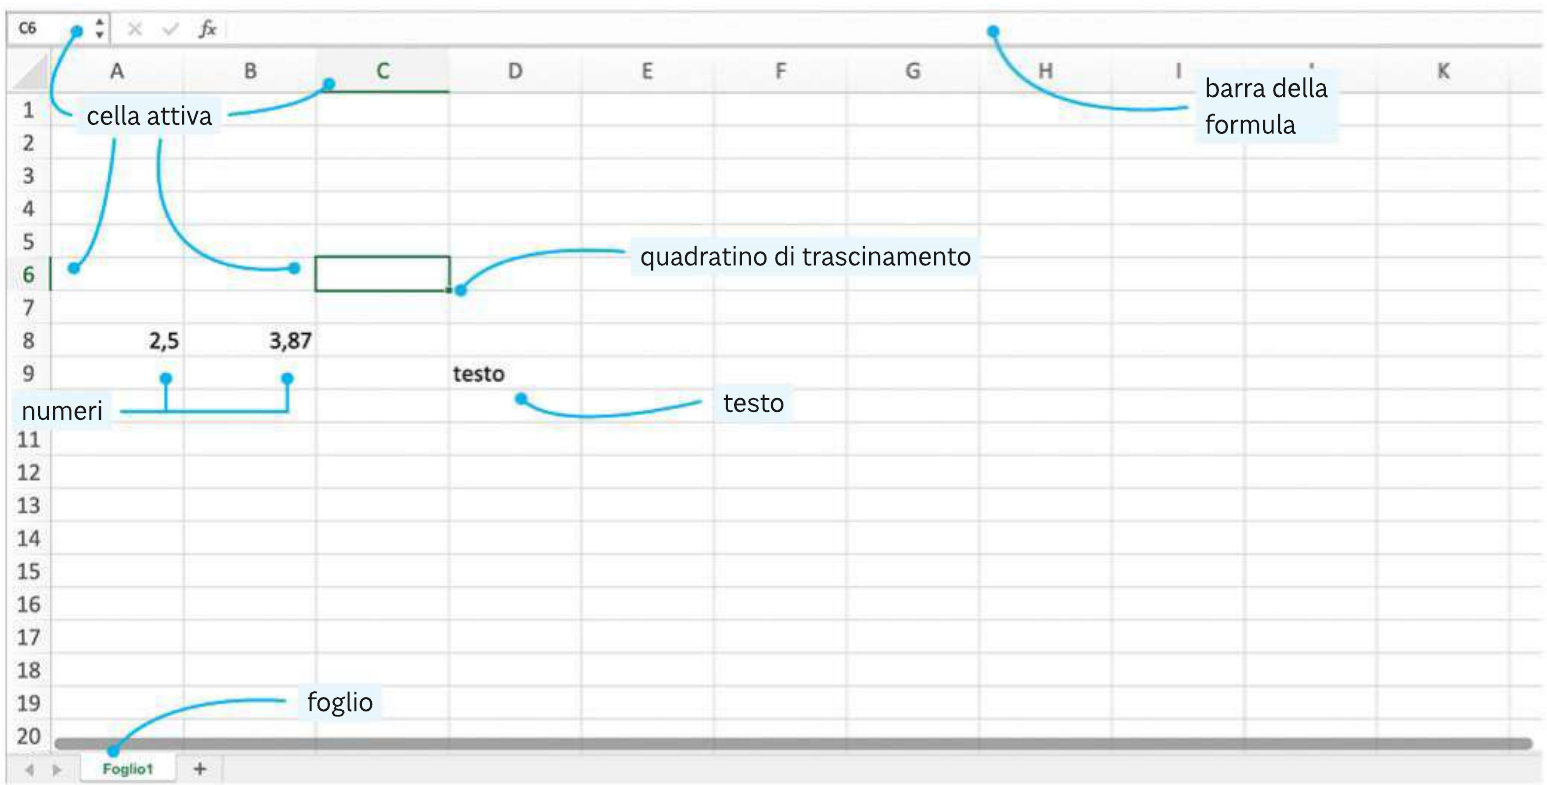
\includegraphics[width=\linewidth]{img/calc.png} 
        \caption{Panoramica foglio di calcolo.}
        \label{fig:librecalc}
    \end{figure} 

\subsection{Inserire e modificare i dati}
\begin{figure}[h!]
    \centering
    
\includegraphics[scale=0.3]{img/tasti.png} 
    \label{fig:tasti}
\end{figure} 

Per scrivere all'interno di una cella, è necessario selezionarla puntandola col mouse e facendo clic su di essa. La cella selezionata si attiva e il suo indirizzo compare nel riquadro in alto a sinistra.
Il testo digitato in una cella viene contemporaneamente riprodotto nella barra della formula. Per confermare l'immissione premiamo \texttt{Invio}, oppure un tasto freccia sulla tastiera che porta a un'altra cella.
Se l'immissione è riconosciuta come testo, viene allineata a sinistra della cella; se è riconosciuta come numero, viene allineata a destra.
Si può selezionare un insieme di celle facendo clic con il mouse sulla prima e, tenendo premuto il pulsante, trascinando il cursore fino all'ultima. Per selezionare gruppi di celle non adiacenti, si seleziona il primo gruppo e poi si procede con i successivi tenendo premuto il tasto CTRL (oppure il tasto Command).

\subsection{Formato di una cella}


Il formato di una cella determina come viene mostrato il suo contenuto.
 Per esempio, se vogliamo visualizzare numeri in notazione scientifica, scegliamo
  il menu \texttt{Formato}, poi \texttt{Celle} e infine, nella finestra di dialogo che comparirà, 
  scegliamo la scheda \texttt{Numeri} e la categoria \texttt{Scientifico} 
  (se digitiamo il numero 0,000005 e premiamo invio, 
  nella cella comparirà $\num{5,00e-6}$).
  Il numero può anche essere inserito direttamente in notazione scientifica,
   per esempio come 3E+6 per indicare $\num{3e+6}$.
  Utilizzando invece il menù \texttt{Formato/Celle/Numero} possiamo scegliere
   quante cifre decimali di ogni numero mostrare, per facilitare
    la lettura e il confronto. I dati sono comunque registrati e utilizzati 
    con tutte le cifre con cui sono stati inseriti o calcolati e 
    la modifica riguarda solo la loro presentazione grafica.
  \begin{figure}[h!]
    \centering
    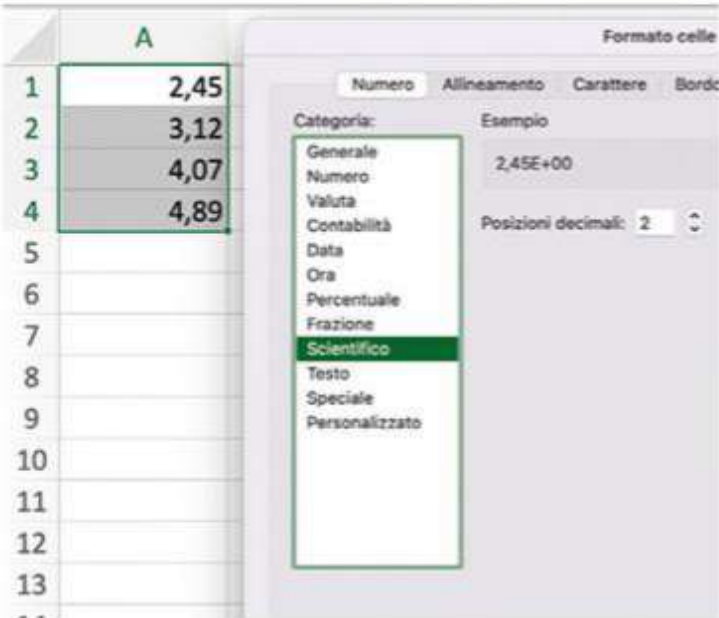
\includegraphics[scale=0.4]{img/formato-cella.png} 
    \caption{Formato in notazione scientifica}
    \label{fig:formatocella}
\end{figure} 

Nella colonna A della figura \ref{fig:insdati} sono stati inseriti quattro numeri decimali, di cui due in notazione scientifica. I numeri sono stati copiati nella colonna B, formattata con due cifre decimali, 
e nella colonna C, formattata in notazione scientifica con una cifra decimale.
\begin{figure}[h!]
    \centering
    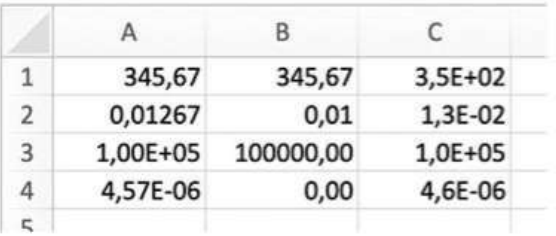
\includegraphics[scale=0.4]{img/inserimento-dati.png} 
    \caption{Inserimento dati}
    \label{fig:insdati}
\end{figure}
\subsection{Inserire e modificare le formule}

\begin{definizione}
Una formula è un'espressione che, digitata in una cella,
 effettua automaticamente dei calcoli o delle operazioni sui dati del 
 foglio di calcolo. Ogni formula deve essere preceduta dal simbolo =.
\end{definizione}

















\begin{testexample}

La cella A2 contiene il valore 2,5 e la cella B2 contiene
 il valore 3,5. Se nella cella C2 digitiamo \texttt{=A2+B2} e premiamo \texttt{Invio}, 
 in essa comparirà il valore 6,
 ossia la somma dei contenuti delle celle A2 e B2.

 \begin{minipage}{\linewidth}
	\centering
    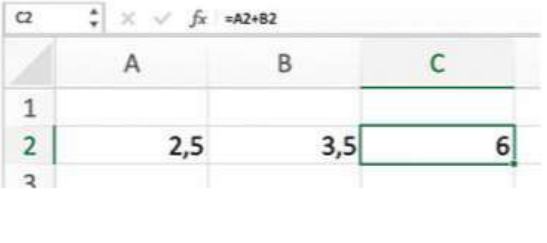
\includegraphics[scale=0.4]{img/inserimento-formula.png} 
	\captionof{figure}{Inserimento formule}
    \label{fig:esempioformule}\end{minipage}
\end{testexample}

\subsubsection{Riferimenti relativi}
Consideriamo la tabella a due colonne rappresentata nella figura \ref{fig:rifrel}. Vogliamo
eseguire il prodotto tra i dati $x$ della colonna A e i corrispondenti dati $y$ della 
colonna B, scrivendo il risultato nella colonna C. Dobbiamo allora eseguire le
seguenti operazioni:
\begin{itemize}
    \item Selezioniamo la cella C2.
    \item Digitiamo la formula = A2*B2.
    \begin{figure}[h!]
        \centering
        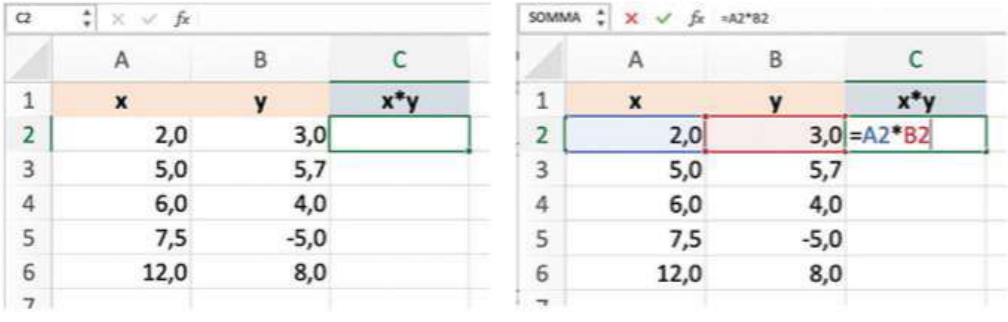
\includegraphics[scale=0.4]{img/riferimenti-relativi.png} 
        \caption{Riferimenti relativi.}
        \label{fig:rifrel}
    \end{figure}
    \item Premiamo \texttt{Invio} nella cella C2 compare il risultato del prodotto.
    \item Selezioniamo di nuovo la cella C2.
    \item Facciamo clic sul quadratino di trascinamento (nell'angolo in basso della cella) e,
    tenendo premuto, lo trasciniamo fino alla cella 6 (i dettagli potrebbero cambiare
    a seconda del foglio di calcolo). Otteniamo la situazione in figura \ref{fig:copyform}
    \begin{figure}[h!]
        \centering
        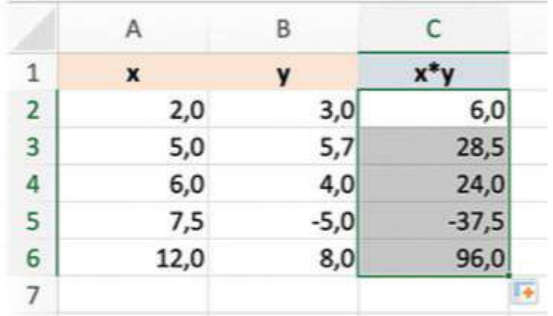
\includegraphics[scale=0.4]{img/copia-formula.png} 
        \caption{}
        \label{fig:copyform}
    \end{figure} 
\end{itemize}
In questo modo, appariranno i prodotti A3*B3 in C3, A4*B4 in C4 e così via. 
Osserviamo dunque che la formula è stata copiata \textit{adattando riga per riga i riferimenti} che, per questa
ragione, sono detti \textit{relativi}.
\subsubsection{Riferimenti assoluti}

Supponiamo ora di voler moltiplicare ciascun dato della colonna A 
per il coefficiente costante $k =  3$, memorizzato nella cella con riferimento E2,
 e scrivere i risultati nella colonna B.

Se seguissimo i passaggi descritti in precedenza, il foglio eseguirebbe i
 seguenti calcoli: A2*E2 in B2, A3*E3 in B3, ecc. Non è quello che vogliamo, 
 perché il secondo fattore deve rimanere sempre E2 in tutta la colonna B.
  Per ottenere questo risultato, è sufficiente ripetere le operazioni 
  descritte in precedenza con la differenza che nel passaggio 2 si deve digitare la
   formula =A2+\$E\$2.
Con l'aggiunta del simbolo \$ nella scrittura si specifica che, in tutti i prodotti,
 il riferimento al contenuto della cella E2 deve rimanere fisso, cioè \textit{assoluto}.

\subsubsection{Ricalcolo automatico}
Proviamo ora a cambiare il dato nella cella E2: inseriamo il valore
2 al posto di 3 e premiamo \texttt{Invio}. Tutti i valori contenuti nella cella B,
che si basano sul valore di E2, si modificano in modo automatico (\ref{fig:ricalcolo}).
\begin{figure}[h!]
    \centering
    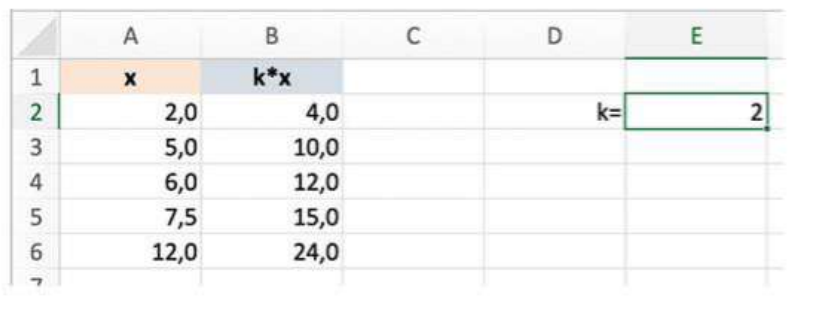
\includegraphics[scale=0.4]{img/ricalcolo.png} 
    \caption{Ricalcolo istantaneo.}
    \label{fig:ricalcolo}
\end{figure} 
Il foglio ha effettuato il \textit{ricalcolo automatico}, utilizzando le formule
introdotte in precedenza nelle celle della colonna B, ma aggiornando il risultato
del prodotto.
\subsubsection{Funzioni integrate}
Un foglio di calcolo, contiene una \textit{Libreria di funzioni}, cioè Formule
predefinite che svolgono automaticamente le operazioni usate più di frequente.
Per esempio, se vogliamo sommare i numeri della colonna B della tabella in figura 
\ref{fig:somma}, possiamo usare la funzione \texttt{SOMMA}.La sintassi di una funzione
è definita dal \textit{nome} e dagli \textit{argomenti}.
\begin{testexample}

    Nella funzione \texttt{SOMMA(B1:B6)}, \texttt{SOMMA} è il nome 
    (ciò che definisce cosa fa la funzione) e \texttt{B1:B6} è \textit{l'argomento}
    (il gruppo di celle coi valori da sommare).
    
     \begin{minipage}{\linewidth}
        \centering
        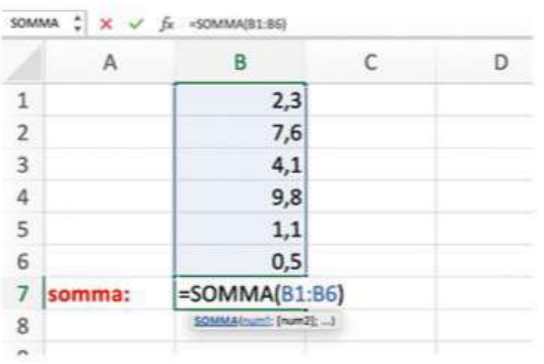
\includegraphics[scale=0.4]{img/somma.png} 
        \captionof{figure}{Funzione somma.}
        \label{fig:somma}\end{minipage}
    \end{testexample}

\subsection{Grafici}
La rappresentazione grafica di una serie di dati è fondamentale per la loro interpretazione: ci permette di cogliere in modo visuale se c'è o meno una correlazione tra due grandezze e di che tipo sia.
Il foglio di calcolo permette di realizzare grafici di diversi tipi, come grafici cartesiani, grafici a barre, areogrammi e istogrammi.
Per l'analisi dei dati raccolti negli esperimenti useremo dei grafici cartesiani, che nel foglio di calcolo si chiamano Grafici a dispersione XY

\subsubsection{Grafici cartesiani}

Un grafico cartesiano rappresenta punti che corrispondono a coppie di valori e si usa per studiare l'eventuale relazione tra due grandezze.
Ecco i passaggi che dobbiamo seguire per costruire un grafico cartesiano a partire dai dati raccolti in una tabella.
\begin{enumerate}
    \item Inseriamo i dati in due colonne adiacenti, scrivendo nella prima
    riga il nome della grandezza e la sua unità di misura. 
    \item Se vogliamo inserire anche le incertezze, dobbiamo distinguere due casi: 
    \item \begin{itemize}
    \item se l'incertezza di una grandezza è la stessa per tutti i dati, 
    possiamo inserirla nella riga di intestazione;

\item se l'incertezza è diversa a seconda dei dati, aggiungiamo una colonna
che riporta l'incertezza di ogni dato.
    \end{itemize}

    \begin{testexample}

    
        
         \begin{minipage}{\linewidth}
            \centering
            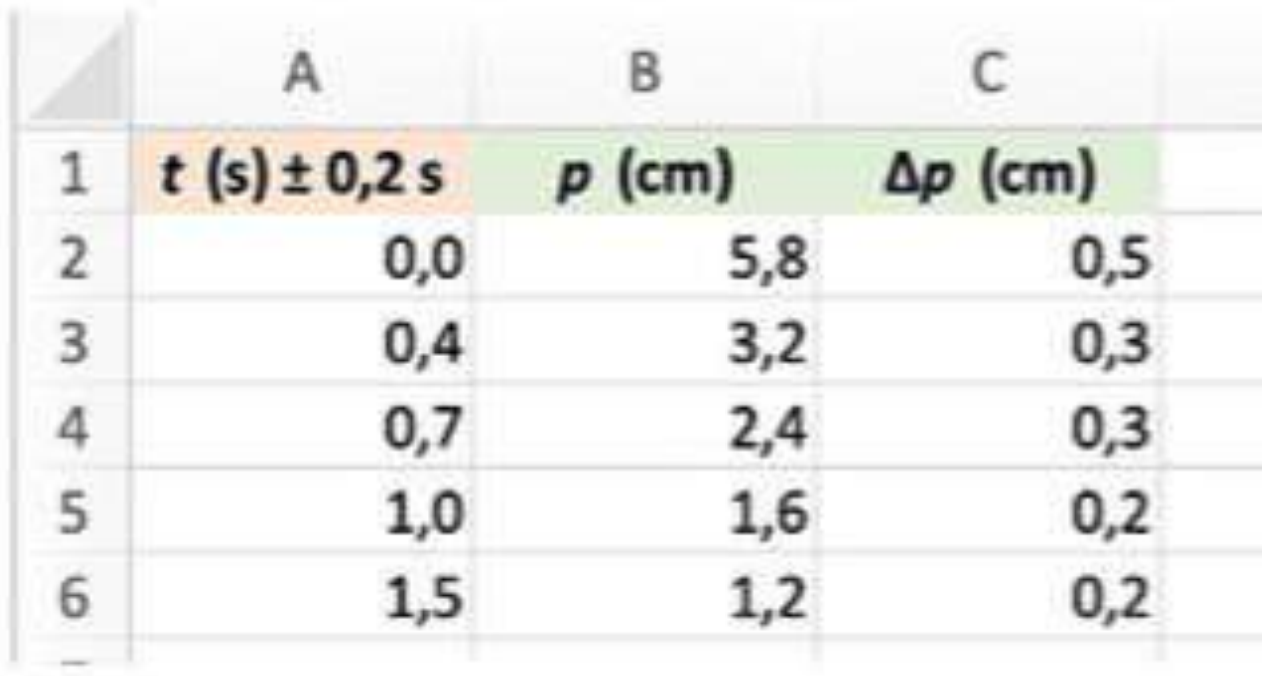
\includegraphics[scale=0.2]{img/barre-libre.png} 
            \captionof{figure}{Inserimento dei dati per il grafico.}
            \label{fig:barrelibre}\end{minipage}
        \end{testexample}

\item Selezioniamo le celle che contengono i dati da rappresentare
(trascuriamo per ora l'eventuale colonna delle incertezze).
\item Seguiamo il percorso \texttt{Inserisci/Ogetto/Grafico} o selezioniamo
direttamente l'icona corrispondente a \texttt{Inserisci grafico}:
appare una finestra di dialogo in cui si può selezionare il tipo di grafico
(anche in questi casi la posizione dei comandi nei menù potrebbe cambiare in
base al programma usato.)
\item Per ottenere un grafico cartesiano, bisogna scegliere \texttt{Dispersione}.
\begin{figure}[h!]
    \centering
    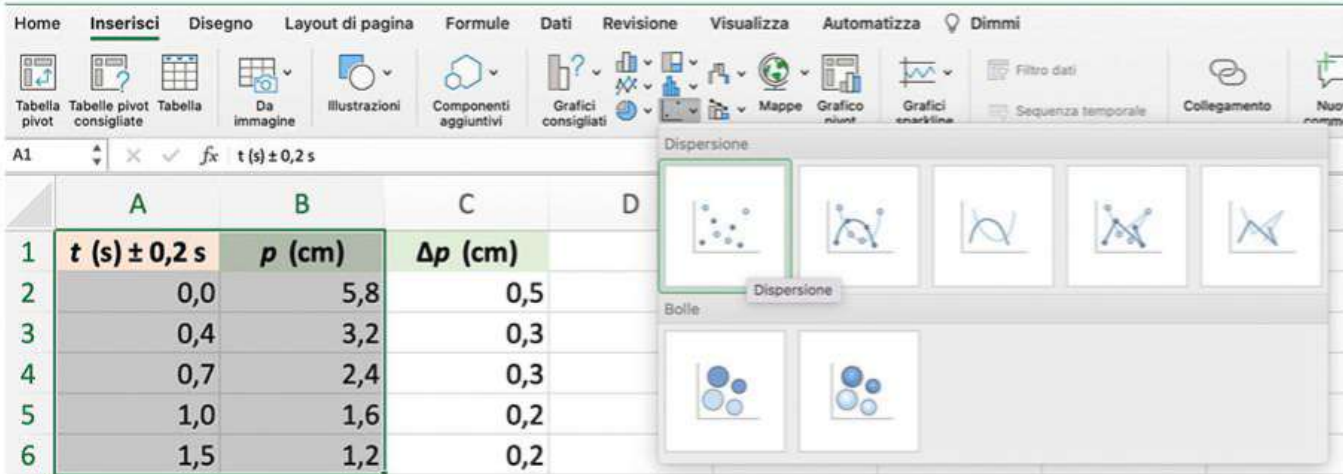
\includegraphics[scale=0.3]{img/dispersione-libreoffice.png} 
    \caption{}
    \label{fig:disperslo}
\end{figure}
\item Scegliamo inoltre di rappresentare solo i punti, senza nessun  tipo di connessione
tra essi. 
\item Modifichiamo il \textit{Titolo del grafico} e aggiungiamo i \textit{Titoli degli assi},
inserendo le grandezze e le rispettive unità di misura.
\item Selezionando con il tasto destro gli assi cartesiani, possiamo inserire la
\textit{griglia secondaria}  ed eventualmente modificare l'intervallo da 
rappresentare su ogni asse.
\begin{figure}[h!]
    \centering
    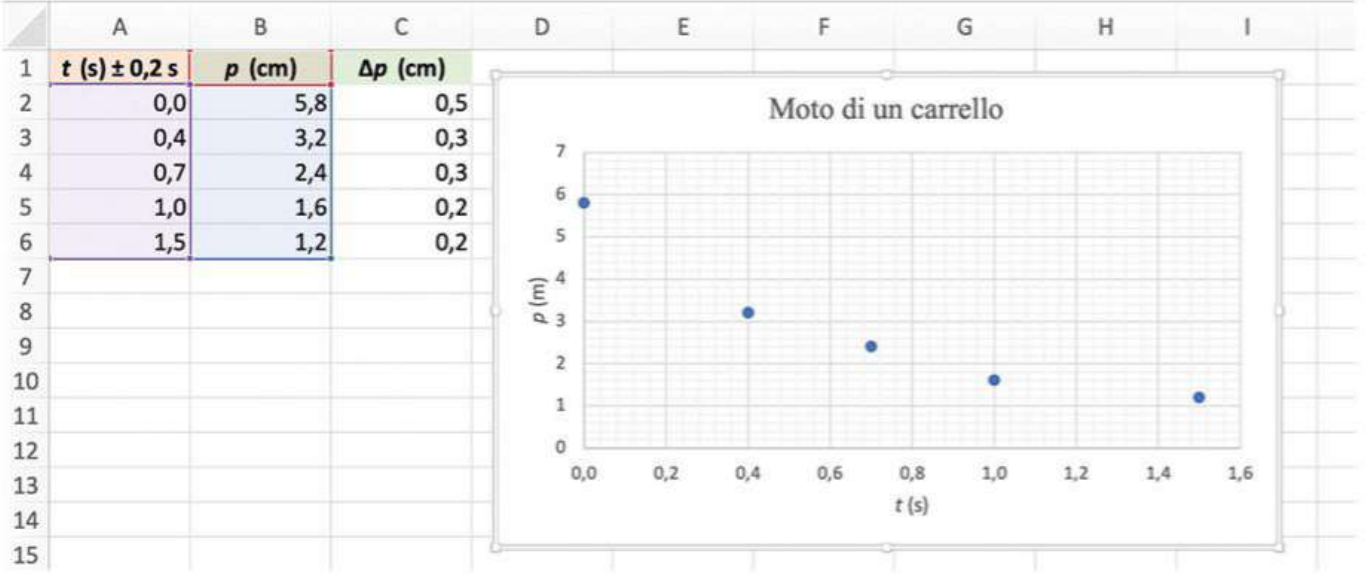
\includegraphics[scale=0.3]{img/grafico-libreoffice.png} 
    \caption{Grafico a dispersione.}
    \label{fig:puntilibre}
\end{figure}
\end{enumerate}

\subsection{Elementi accessori per l'analisi dei dati}
Ai grafici è possibile aggiungere alcuni elementi che ci aiutano ad 
analizzare i dati, come le \textit{barre di errore} e le \textit{linee di tendenza}. 

\begin{definizione}
    Le barre di errore ci permettono di visualizzare in modo grafico le incertezze nelle
    misure raccolte.
\end{definizione}
Possiamo chiedere al foglio di calcolo di mostrare le barre di errore  sul grafico.

\begin{itemize}
    \item Selezioniamo i punti sul grafico con il tasto destro del mouse.
    \item Si apre un menù specifico per inserire le incertezze. Bisogna specificare
    se l'incertezza è la stessa per tutti i dati o se si vuole selezionare 
    una colonna con le diverse incertezze. 
\end{itemize}
In alternativa, è possibile inserire le barre di errore seguendo il percorso
\texttt{Struttura grafico/Aggiungi elemento  grafico/Barre d'errore.} In 
\texttt{Altre opzioni barre d'errore} è possibile stabilire nel dettaglio 
i valori da assegnare alle barre su entrambi gli assi.
\begin{remark}
    Se le barre sono troppo piccole per essere visualizzate, non le inserire
    nel grafico ma fa in modo che gli errori siano scritti altrove, per esempio nella
    tabella di raccolta e di elaborazione dei dati. Così, chi legge, può sempre
    trovare l'informazione sugli errori nella tua relazione.
\end{remark}

\begin{testexample}

    In questo grafico abbiamo impostato la stessa incertezza su tutte le misure 
    di tempo in ascissa e un'incertezza variabile per le misure in ordinata.
    
     \begin{minipage}{\linewidth}
        \centering
        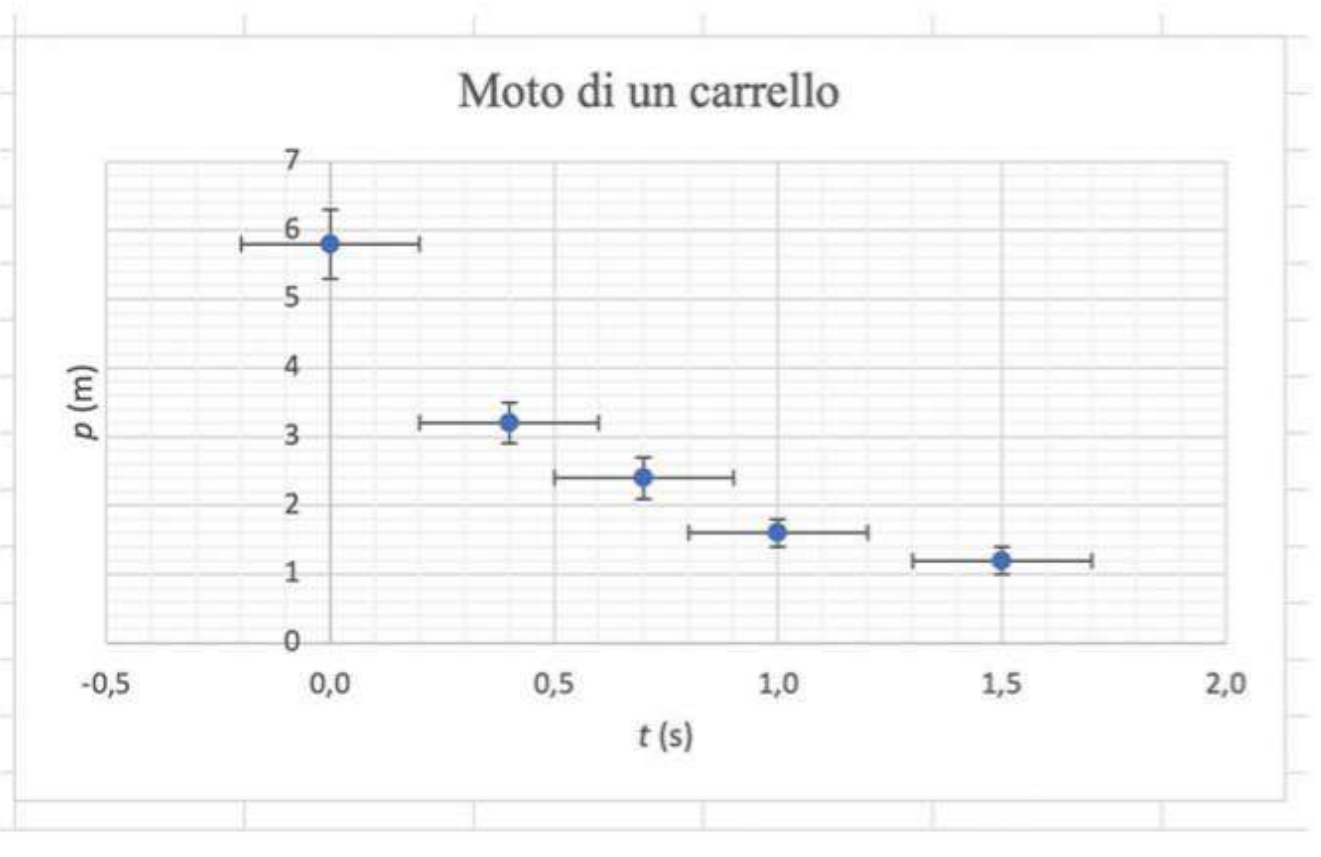
\includegraphics[scale=0.3]{img/moto-carrello-libre.png} 
        \captionof{figure}{Esempio di grafico con barre di errore.}
        \label{fig:motocarrellolibre}\end{minipage}
    \end{testexample}

\subsubsection{Linea di tendenza}

\begin{definizione}
    La linea di tendenza è la curva (o la retta) che meglio approssima i dati
    rappresentati.
\end{definizione}

Possiamo chiedere al foglio elettronico di tracciare la linea di tendenza e 
scriverne l'equazione. 
\begin{enumerate}
    \item Quando il grafico è attivo, clicchiamo col tasto destro sui punti e 
    selezioniamo \texttt{Aggiungi linea di tendenza}. 
    \item Nella finestra di dialogo che si apre, scegliamo \texttt{Visualizza l'equazione sul grafico}. 
    \item Se riteniamo chela relazione sia di proporzionalità diretta (e non 
    semplicemente una relazione lineare), selezioniamo anche l'opzione 
    \texttt{Imposta intercetta 0,0}. 
\end{enumerate}

\begin{testexample}

    In questo grafico è stata selezionata una linea di tendenza senza fissare un valore
    dell'intercetta. L'equazione della retta è visualizzata sul grafico.
    
     \begin{minipage}{\linewidth}
        \centering
        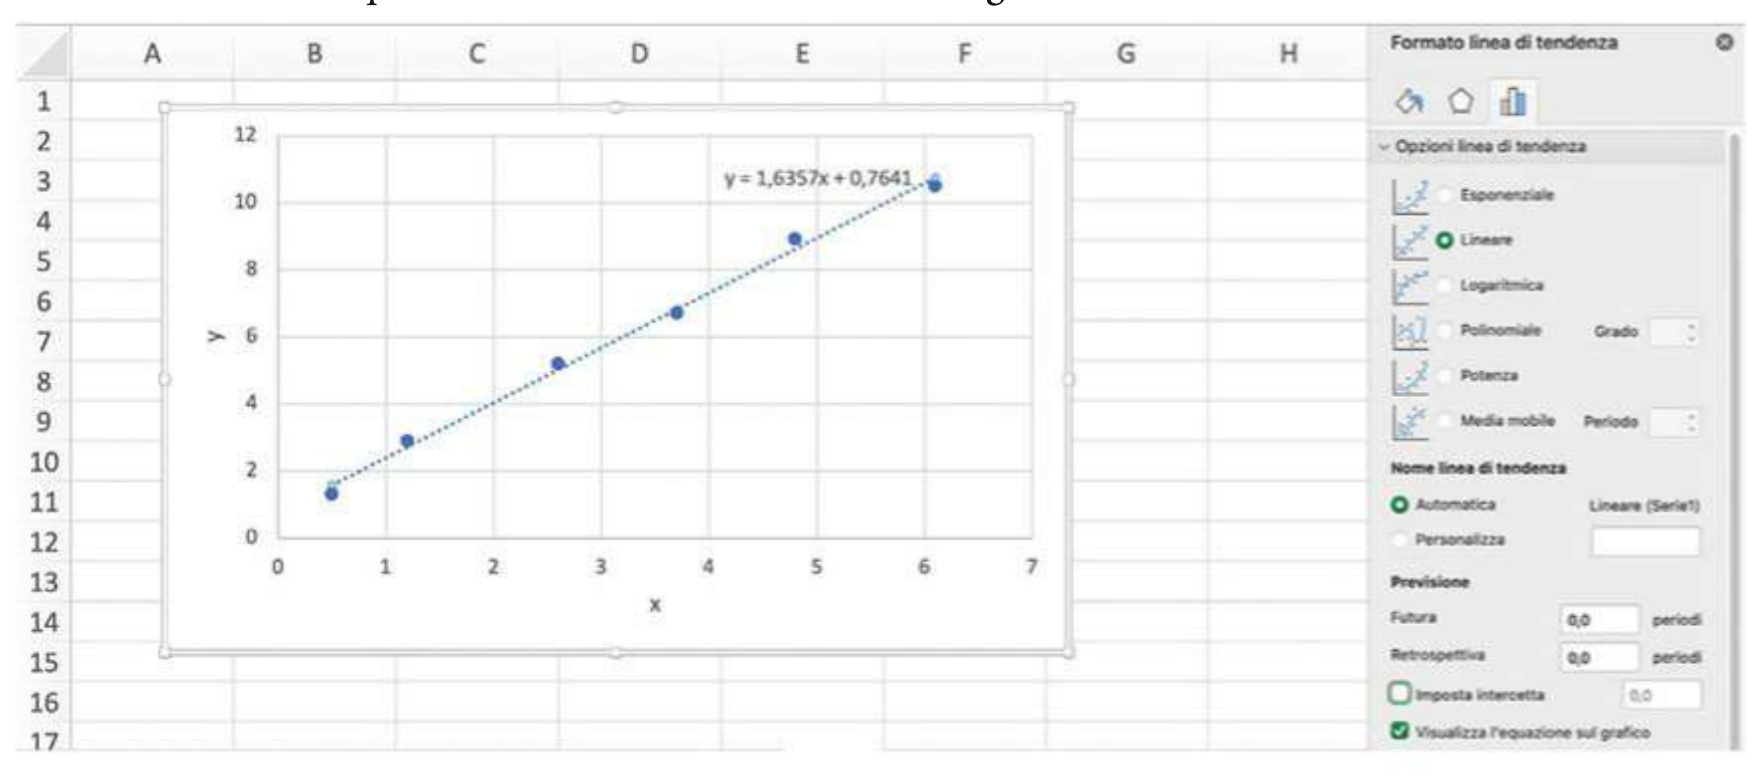
\includegraphics[scale=0.2]{img/linea-tendenza-libre.png} 
        \captionof{figure}{Linea di tendenza lineare.}
        \label{fig:libretendenza}\end{minipage}
    \end{testexample}


\section{Uso dei fogli Google}
In questa sezione, impareremo come creare un grafico a dispersione utilizzando Google Sheets. Seguendo passo per passo, vedremo come inserire i dati, creare il grafico, personalizzarlo con titolo e etichette, e aggiungere una linea di tendenza. Infine, vedremo come mostrare due grafici contemporaneamente.



\subsection{Creazione del Documento}
\begin{enumerate}
    \item Apri Google Sheets e crea un nuovo foglio di calcolo.
    
\begin{figure}[h!]
    \centering
    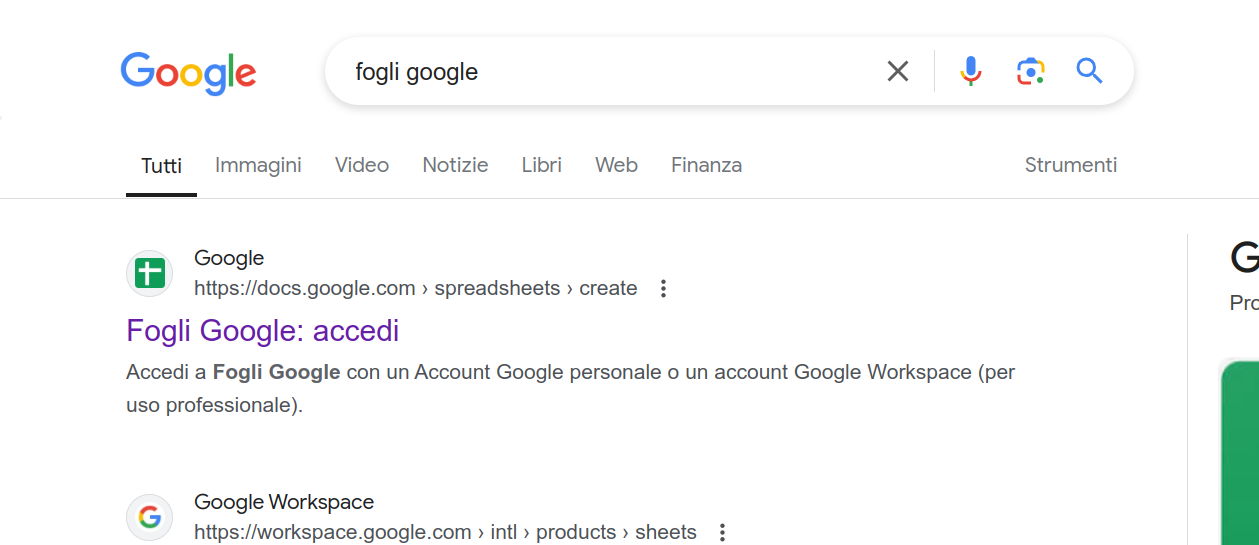
\includegraphics[width=\linewidth]{img/creadoc.png} 
    \caption{Creazione del documento in Google Sheets}
\end{figure}    
    
    \item Rinomina il foglio in modo appropriato, ad esempio, \textit{Esperimento di Fisica} (figura \ref{fig:rinomina}).
    \begin{figure}[h!]
    \centering
    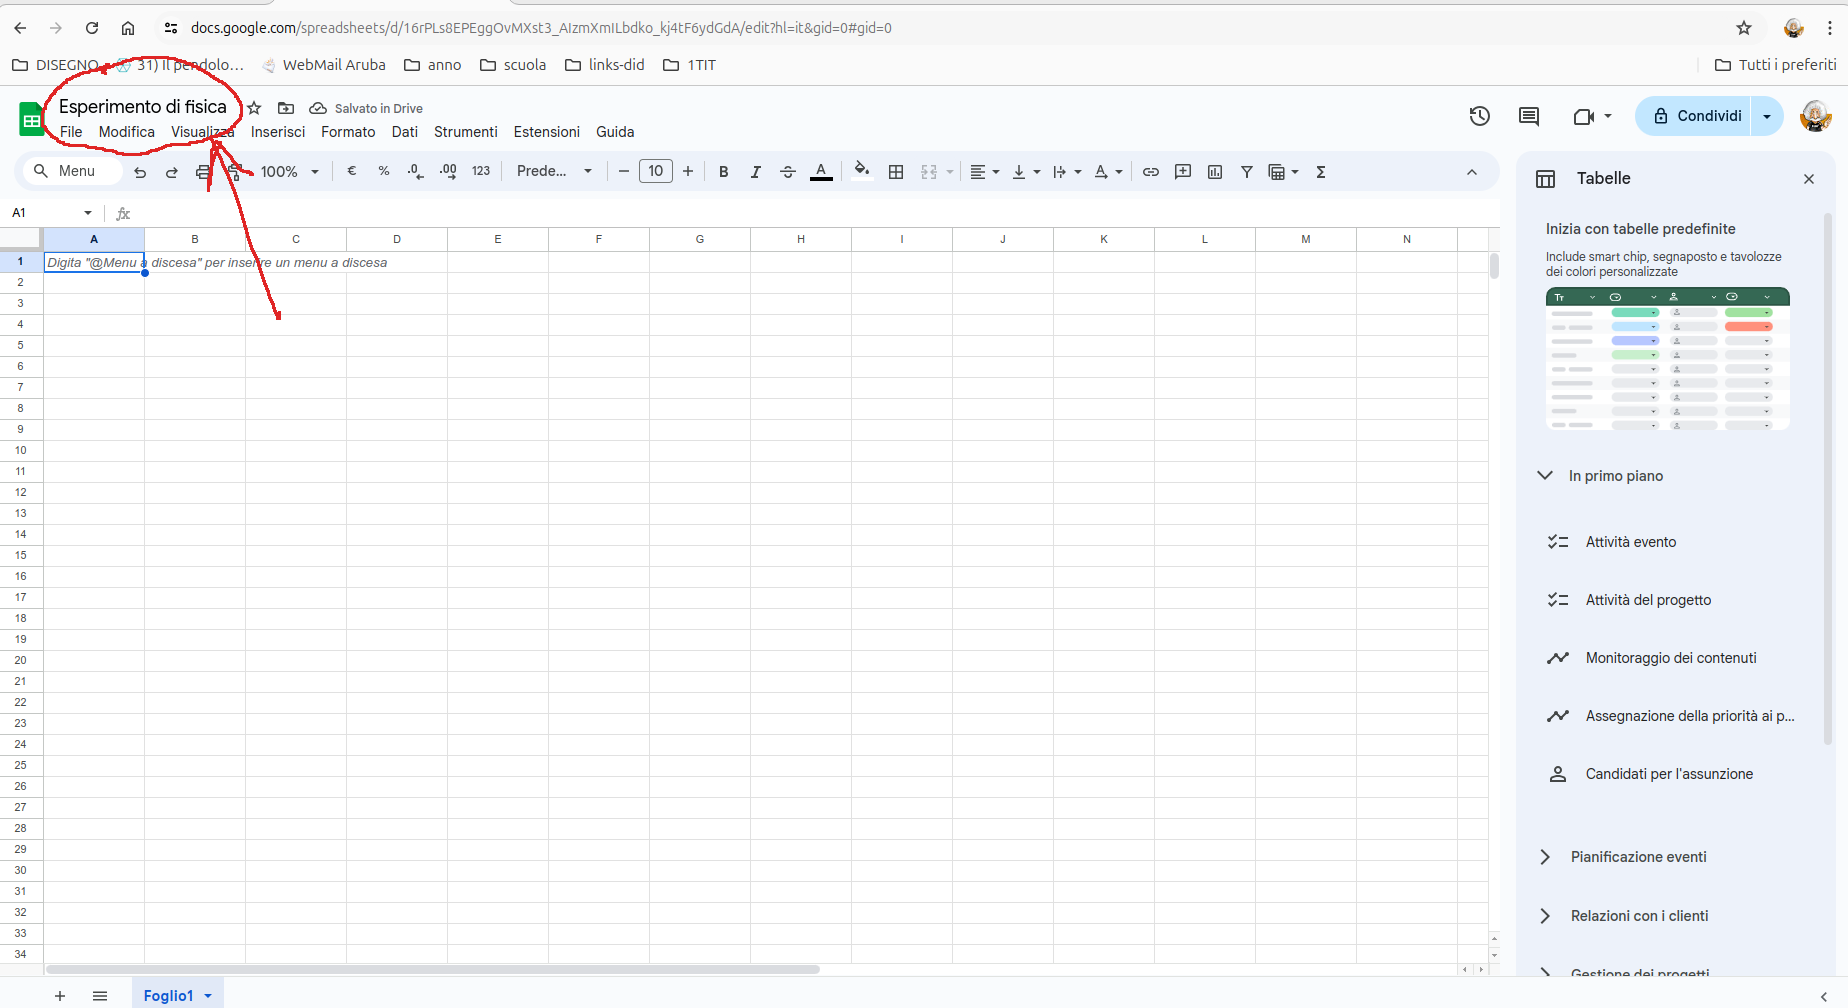
\includegraphics[width=\linewidth]{img/rinomina.png} 
    \caption{Rinomina il  documento in Google Sheets}
    \label{fig:rinomina}
\end{figure} 
\end{enumerate}


\subsection{Inserimento dei dati}
\begin{enumerate}
    \item Inserisci i dati nelle colonne A e B. Ad esempio, nella colonna A metti i valori della variabile indipendente (ad esempio, tempo in secondi), e nella colonna B i valori della variabile dipendente (ad esempio, distanza in metri) (figura \ref{fig:dati}).
    \item Digita i dati manualmente, facendo clic su una cella e digitando il valore. Premi \textbf{Invio} per passare alla cella sottostante.
    \item Esempio di dati:
    \begin{center}
    \begin{tabular}{|c|c|}
    \hline
    Tempo (s) & Distanza (m) \\
    \hline
    1 & 1,2 \\
    2 & 2,5 \\
    3 & 3,1 \\
    4 & 4,0 \\
    5 & 5,3 \\
    \hline
    \end{tabular}
    \end{center}
\end{enumerate}
    \begin{figure}[h!]
    \centering
    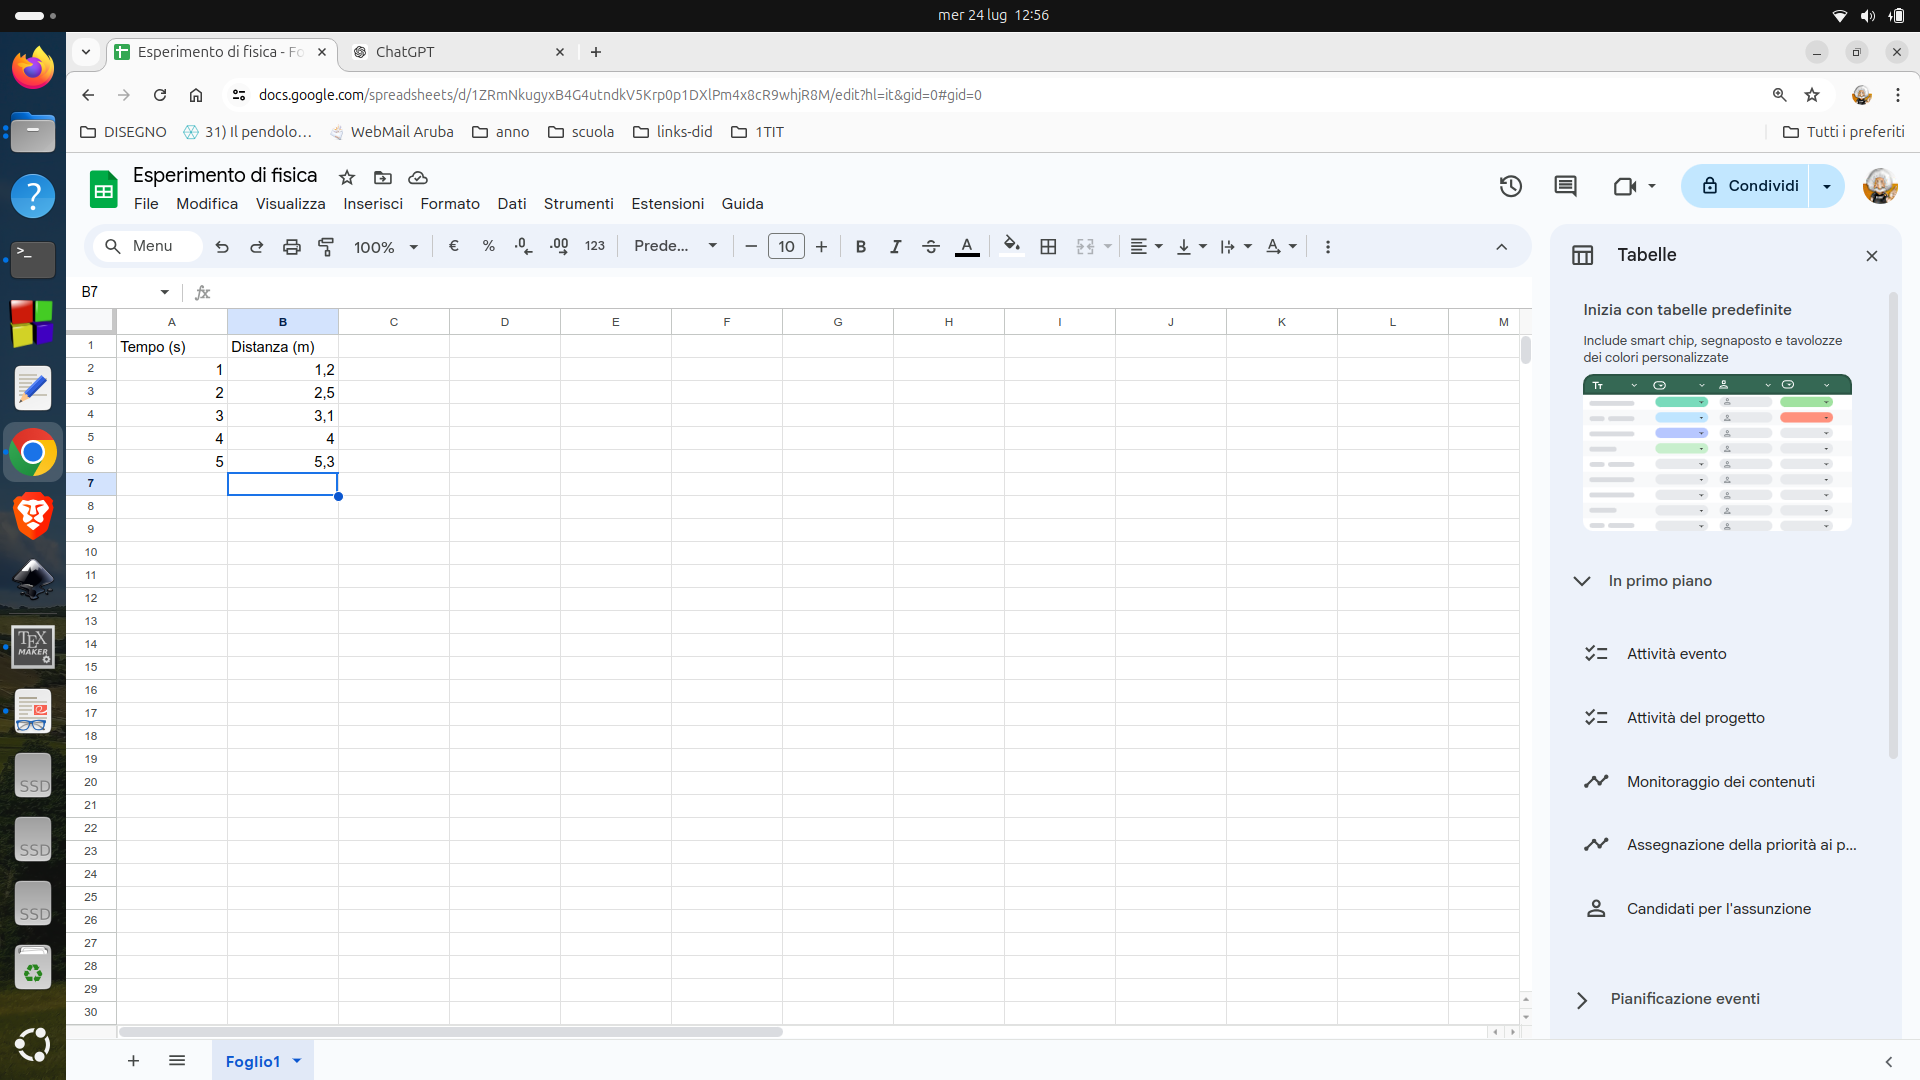
\includegraphics[width=\linewidth]{img/dati.png} 
    \caption{Inserimento dei dati.}
    \label{fig:dati}
\end{figure} 

Da notare che Google Sheets (``fogli di calcolo'', in italiano) utilizza le virgole per i numeri decimali (esattamente come facciamo noi). Altri programmi (e calcolatrici) invece, usano i puntini. Vi accorgete che il foglio di calcolo considera effettivamente scritte come 1,2 come numeri, perché li allinea a destra nella cella.


\subsection{Creazione del Grafico a Dispersione}
\begin{enumerate}
    \item Seleziona i dati inseriti nelle colonne A e B. Puoi farlo cliccando e trascinando il mouse dall'angolo superiore sinistro (A1) all'angolo inferiore destro (B5) dei tuoi dati (figura \ref{fig:selezione}).
     \begin{figure}[h!]
    \centering
    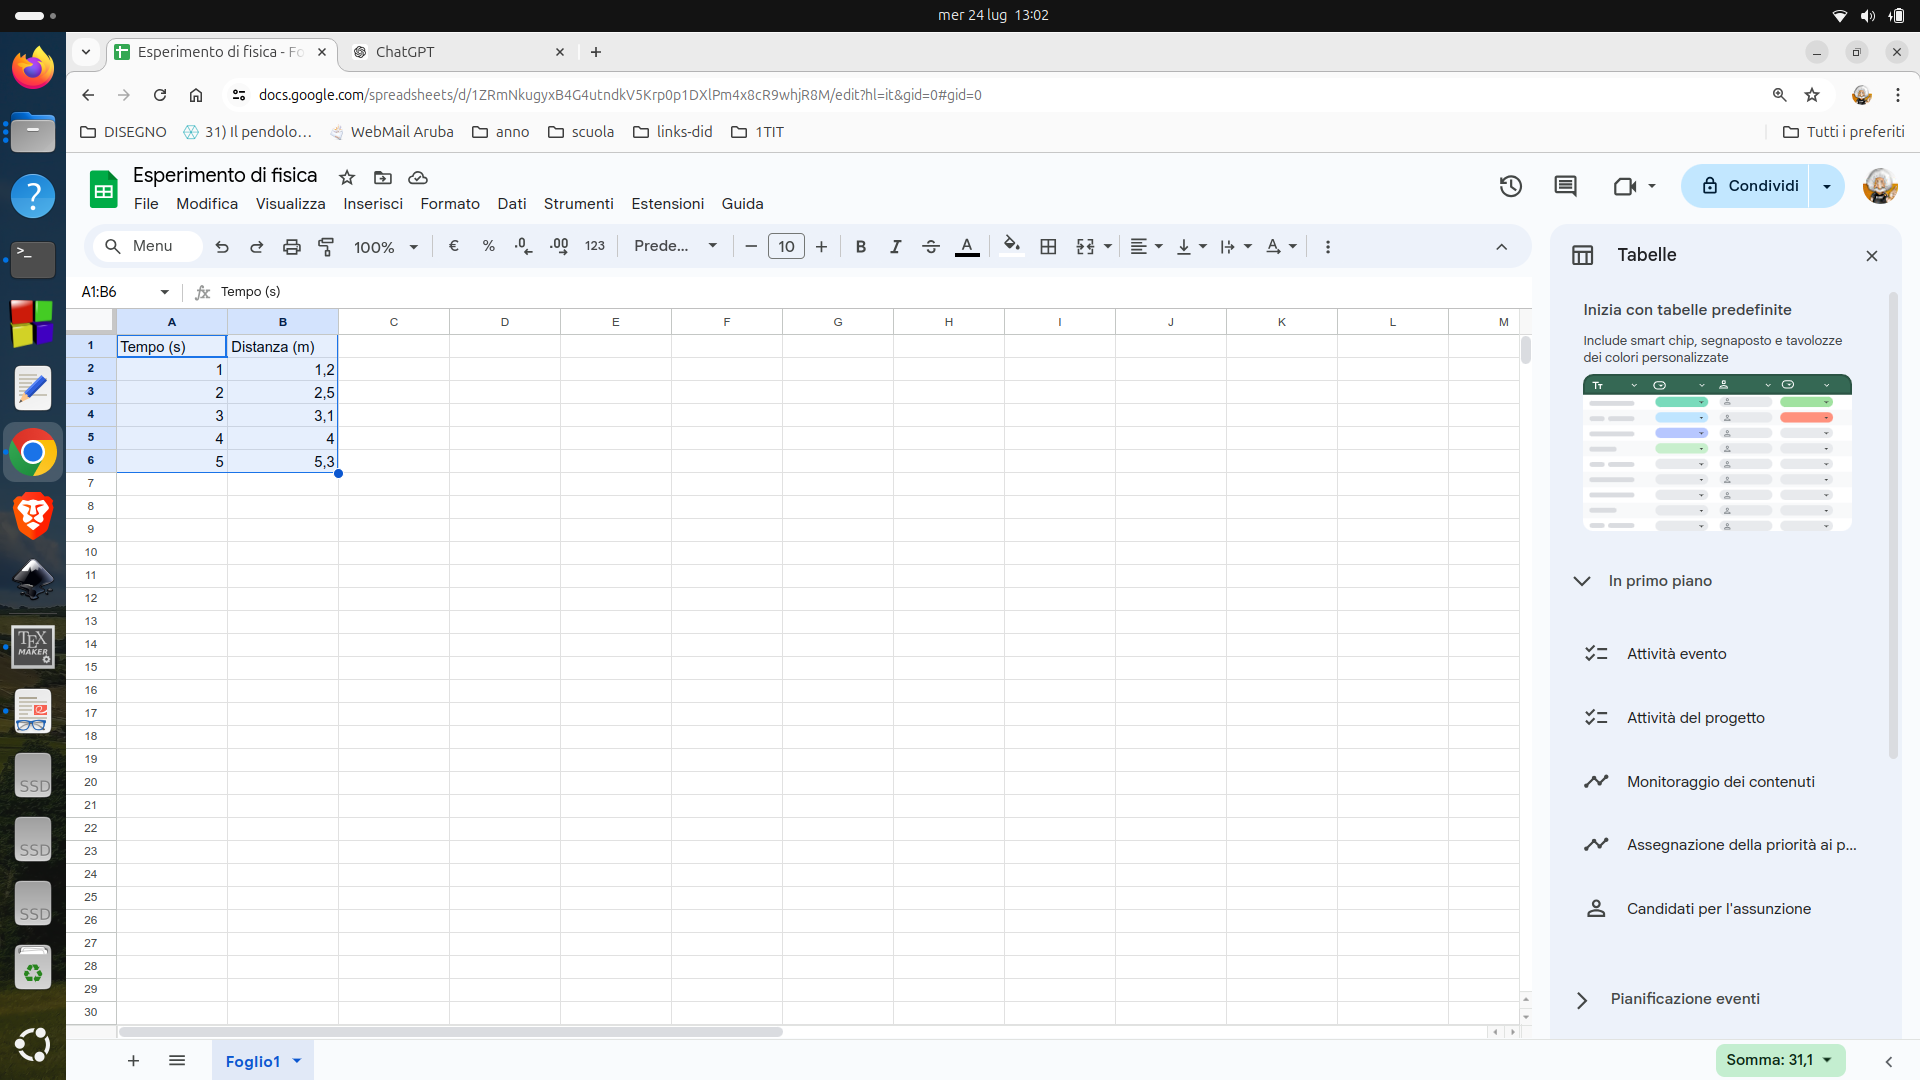
\includegraphics[width=\linewidth]{img/selezione.png} 
    \caption{Seleziome dei dati.}
    \label{fig:selezione}
\end{figure} 
    
    
    \item Vai su \textbf{Inserisci} nel menu e seleziona \textbf{Grafico} (figura \ref{fig:insgrafico}).
    
        \begin{figure}[h!]
    \centering
    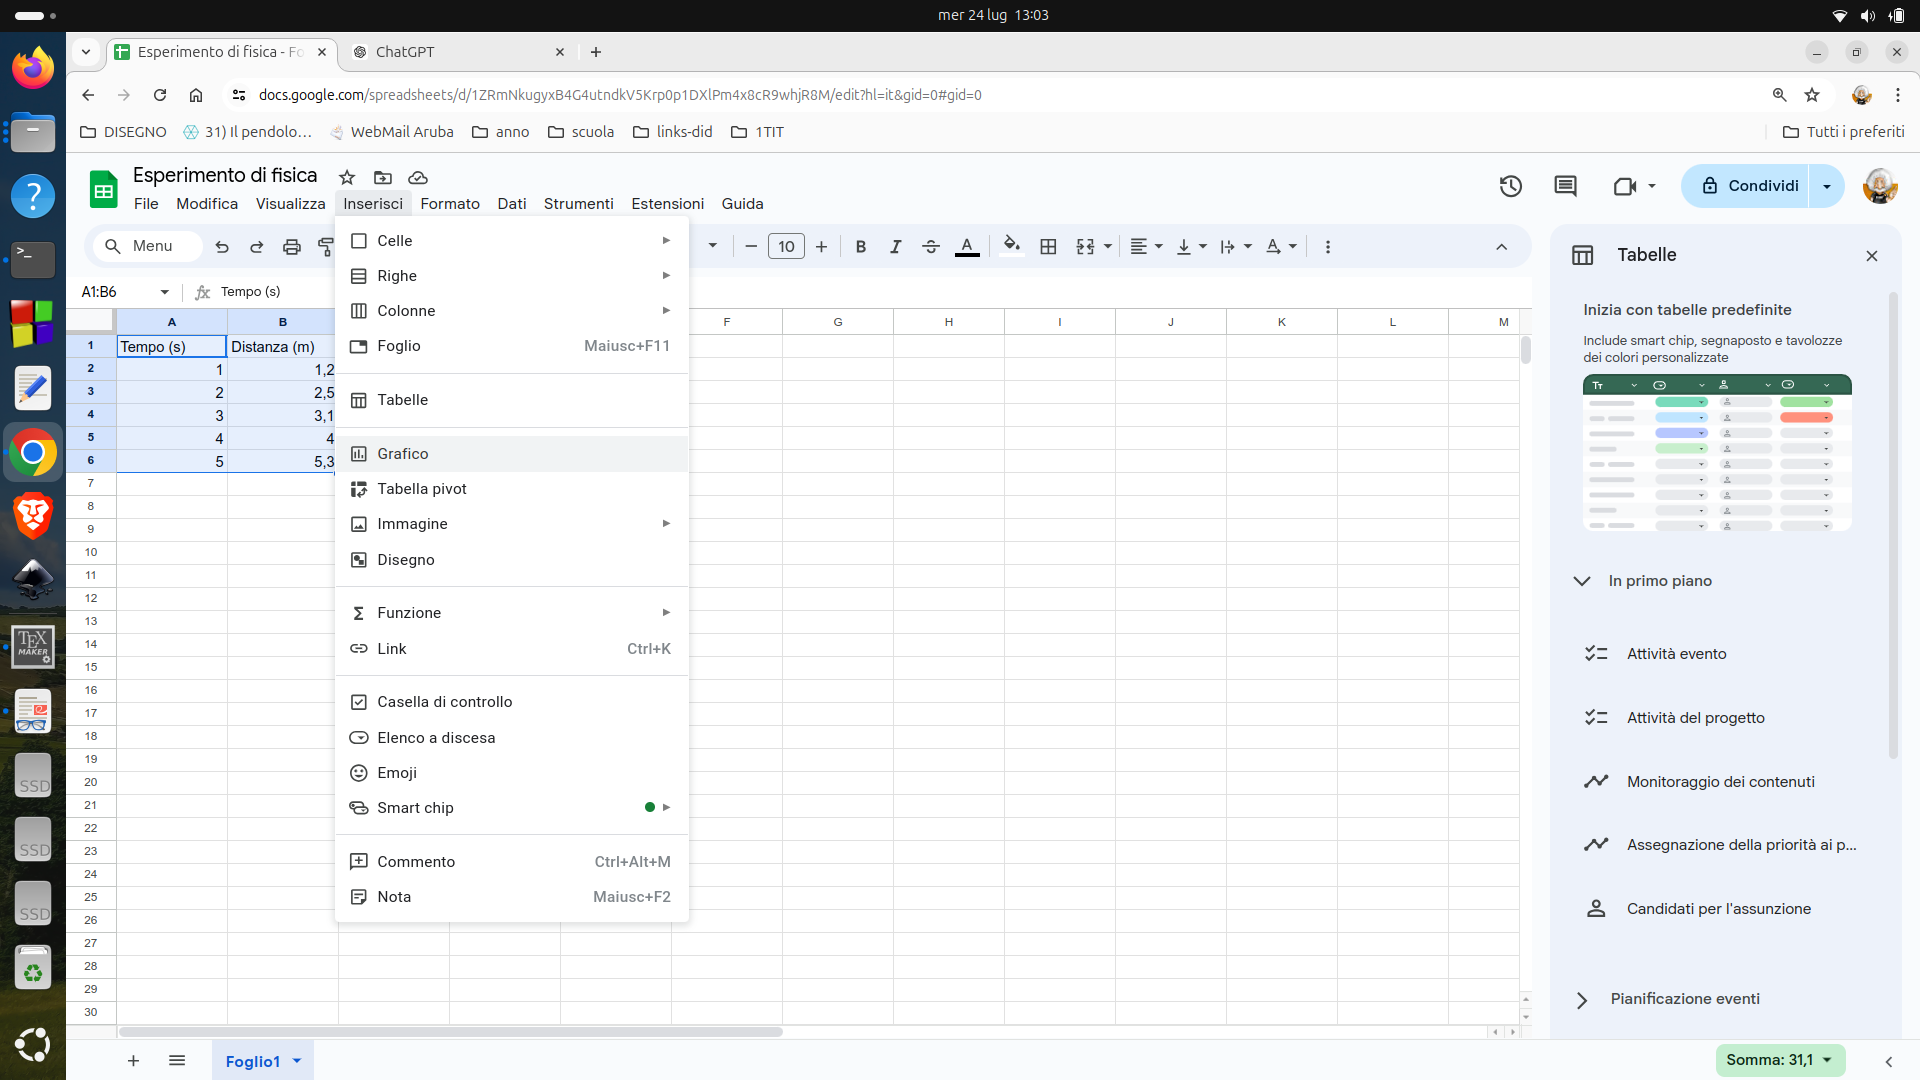
\includegraphics[width=\linewidth]{img/inseriscigrafico.png} 
    \caption{Inserimento del grafico.}
    \label{fig:insgrafico}).
\end{figure}  
    
    
    
    \item Nella finestra delle opzioni del grafico, seleziona \textbf{Grafico a dispersione} dal menu a tendina \textbf{Tipo di grafico} (figura \ref{fig:dispersione}).
    
   \begin{figure}[h!]
    \centering
    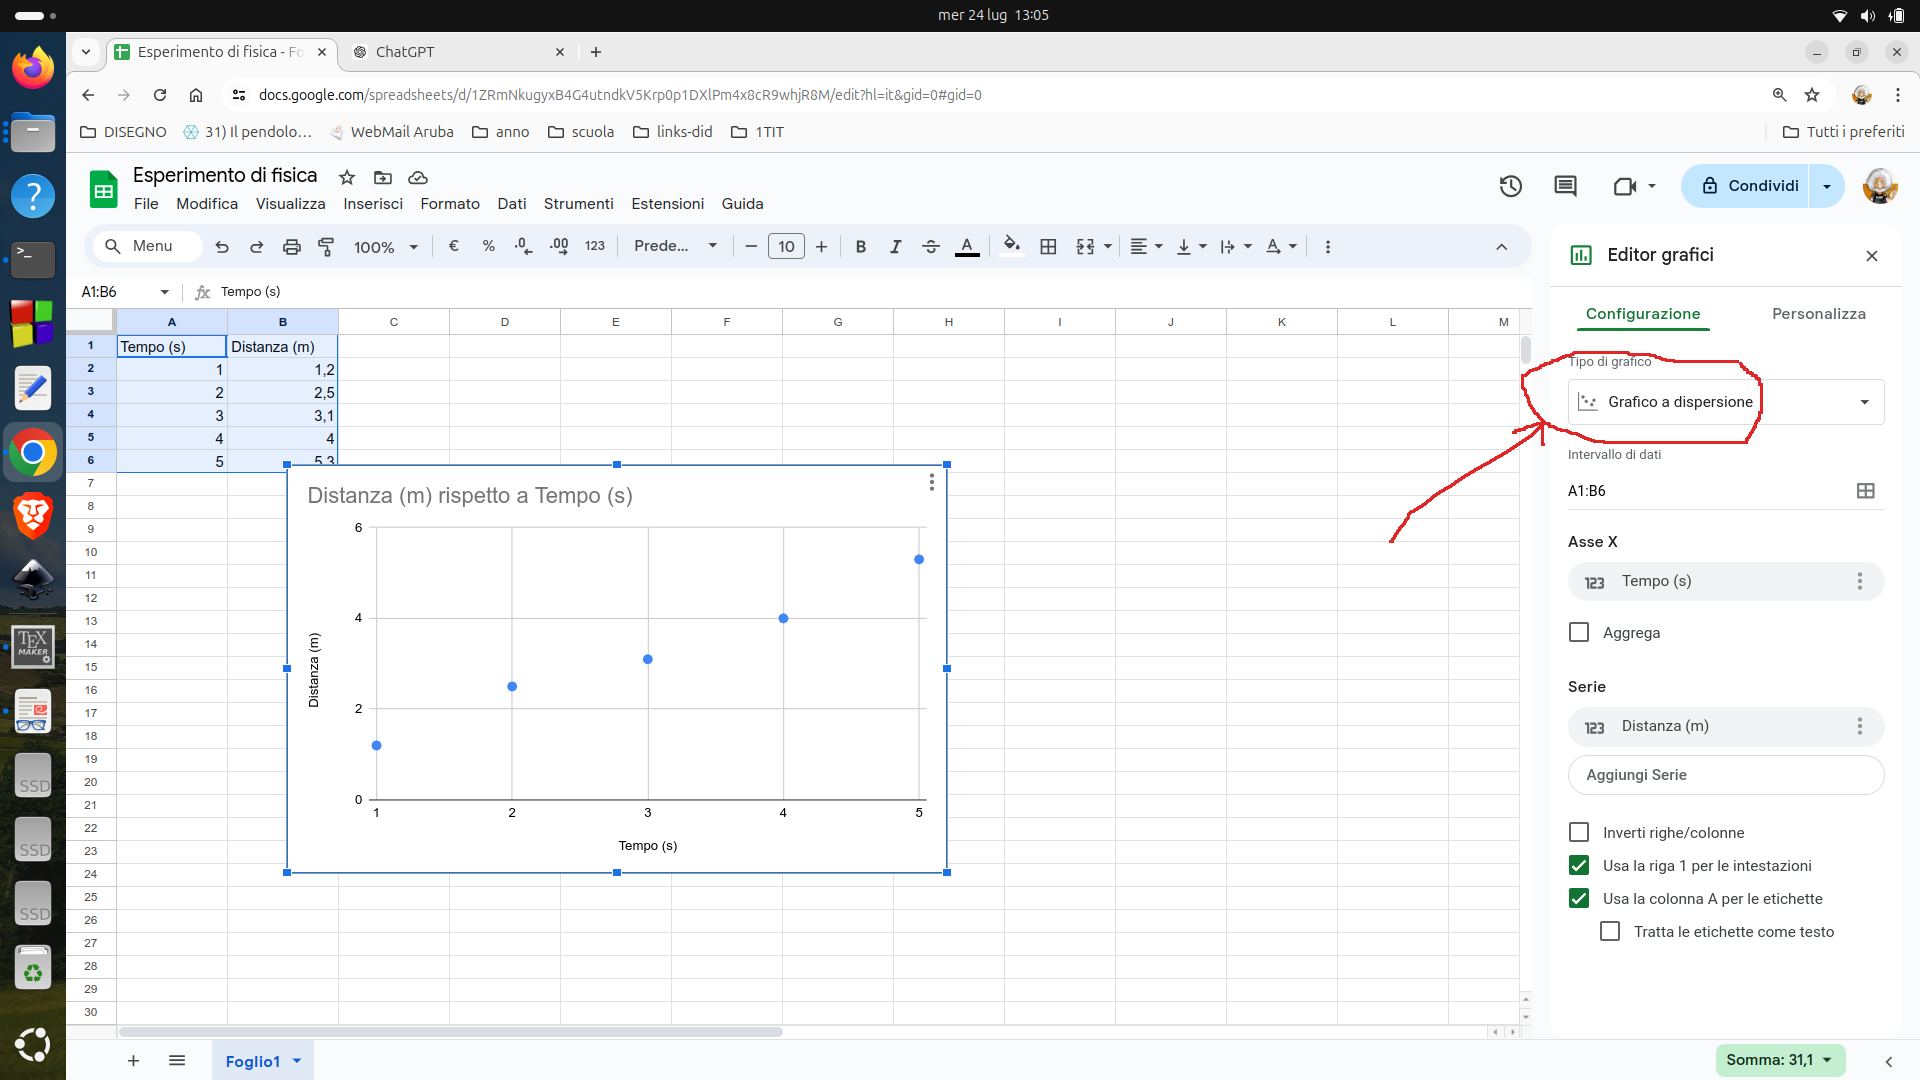
\includegraphics[width=\linewidth]{img/dispersione.png} 
    \caption{Grafico a dispersione.}
            \label{fig:dispersione}
\end{figure} 
\end{enumerate}



\subsection{Personalizzazione del Grafico}
\begin{enumerate}
    \item Per personalizzare il grafico, devi aprire la finestra di modifica (a destra). Se non è già visibile, clicca i tre puntini sul grafico e scegli \textbf{modifica}. Se non vedi i tre puntini, clicca su un'area bianca sul grafico (non sul foglio di calcolo, proprio sul grafico):
    
    \begin{figure}[h!]
    \centering
    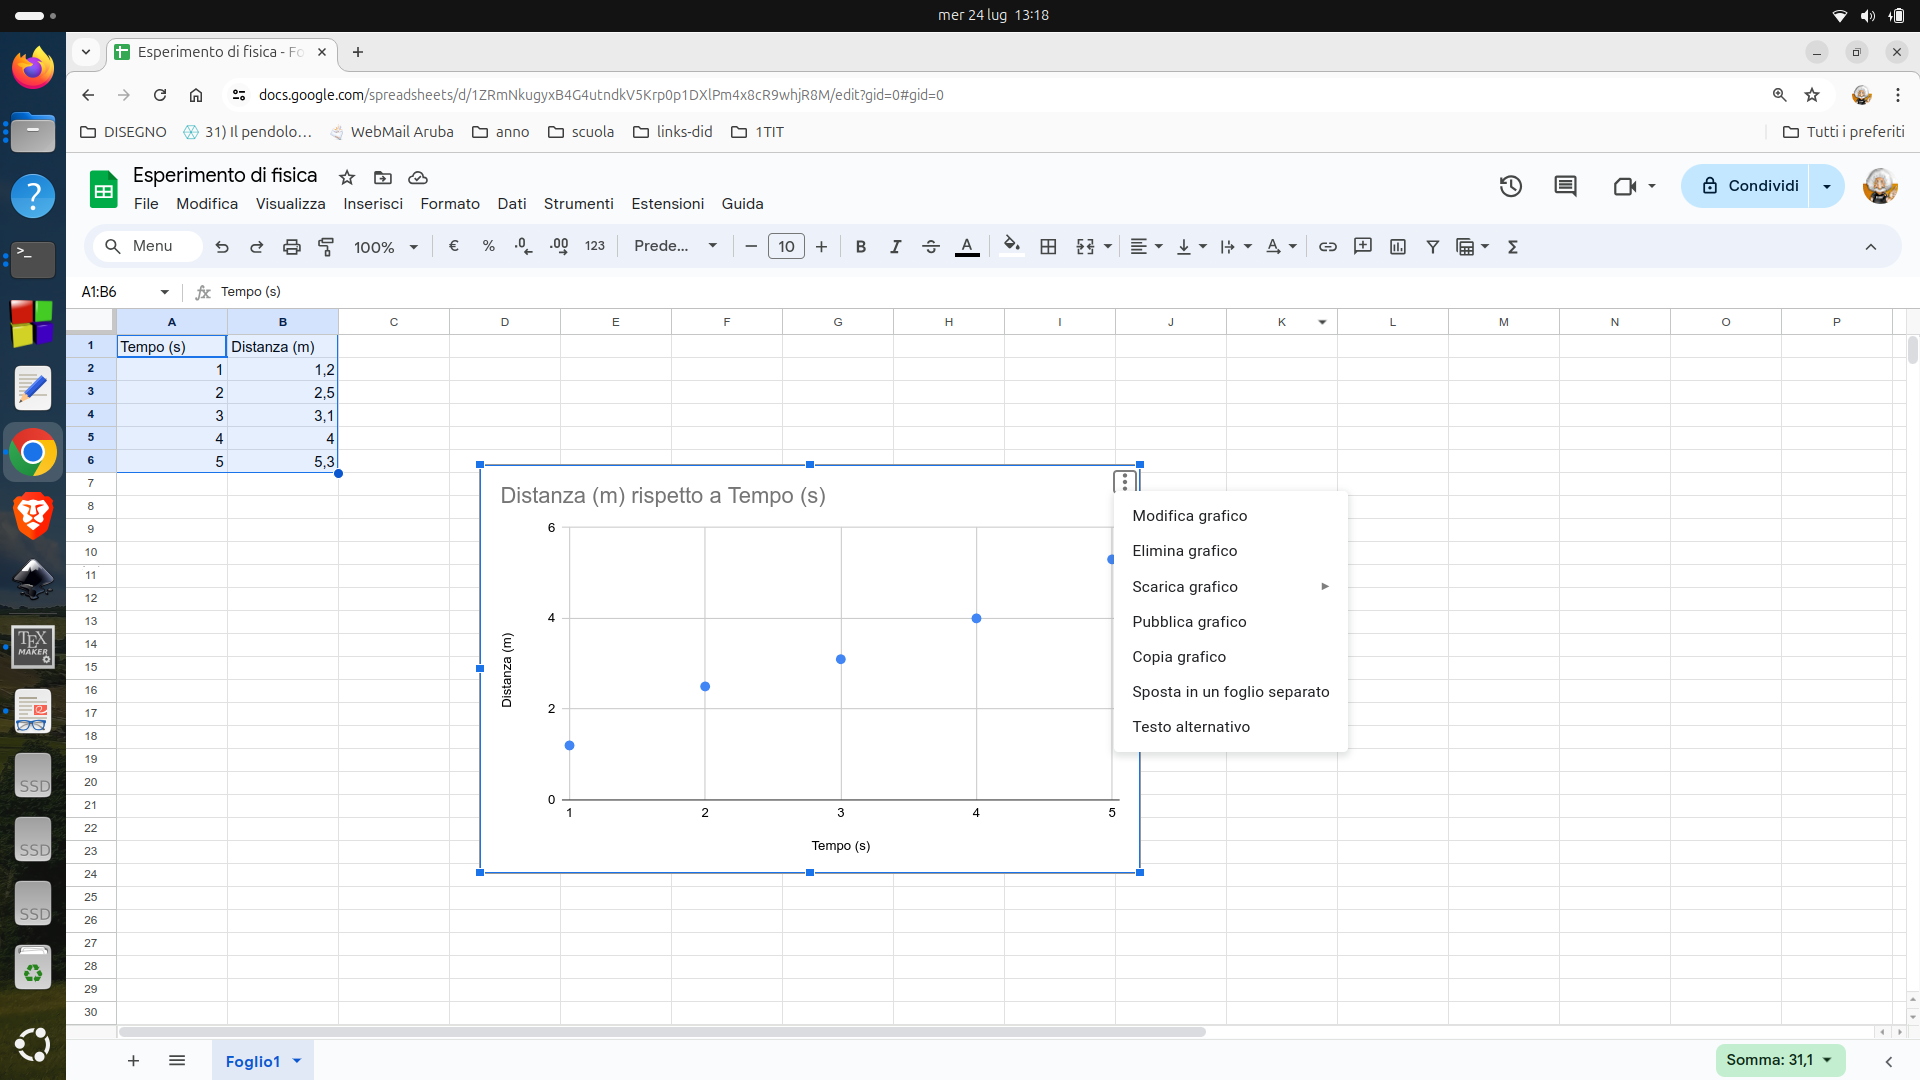
\includegraphics[width=\linewidth]{img/modifica.png} 
    \caption{Modifica del grafico.}
\end{figure} 
    
    \item Clicca sulla scheda \textbf{personalizza} (figura \ref{fig:personalizza})
    \begin{figure}[h!]
    \centering
    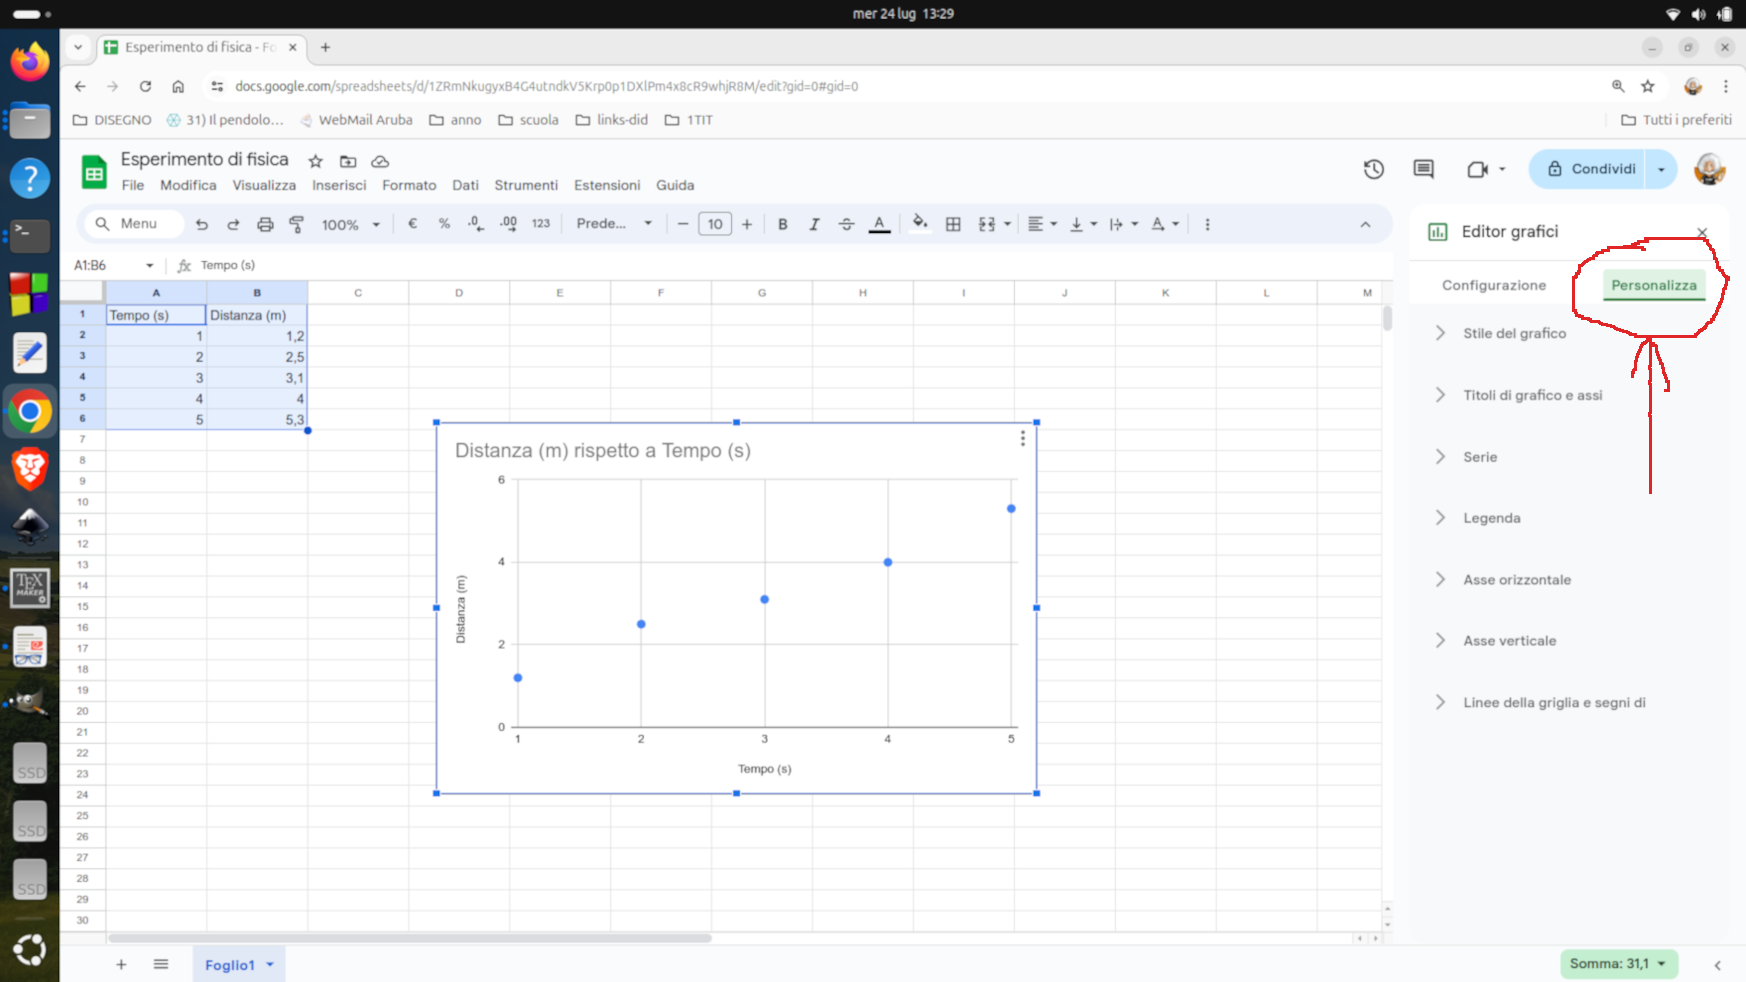
\includegraphics[width=\linewidth]{img/personalizza.png} 
    \caption{Scheda \textbf{Scheda personalizza.}}
    \label{fig:personalizza}
\end{figure} 
    
    
    \item Aggiungi il titolo del grafico: ad esempio, \textit{Relazione tra Tempo e Distanza}: espandendo il sottomenu \textbf{Titolo di grafico e assi} figura \ref{fig:titolo}:
    
 \begin{figure}[h!]
    \centering
    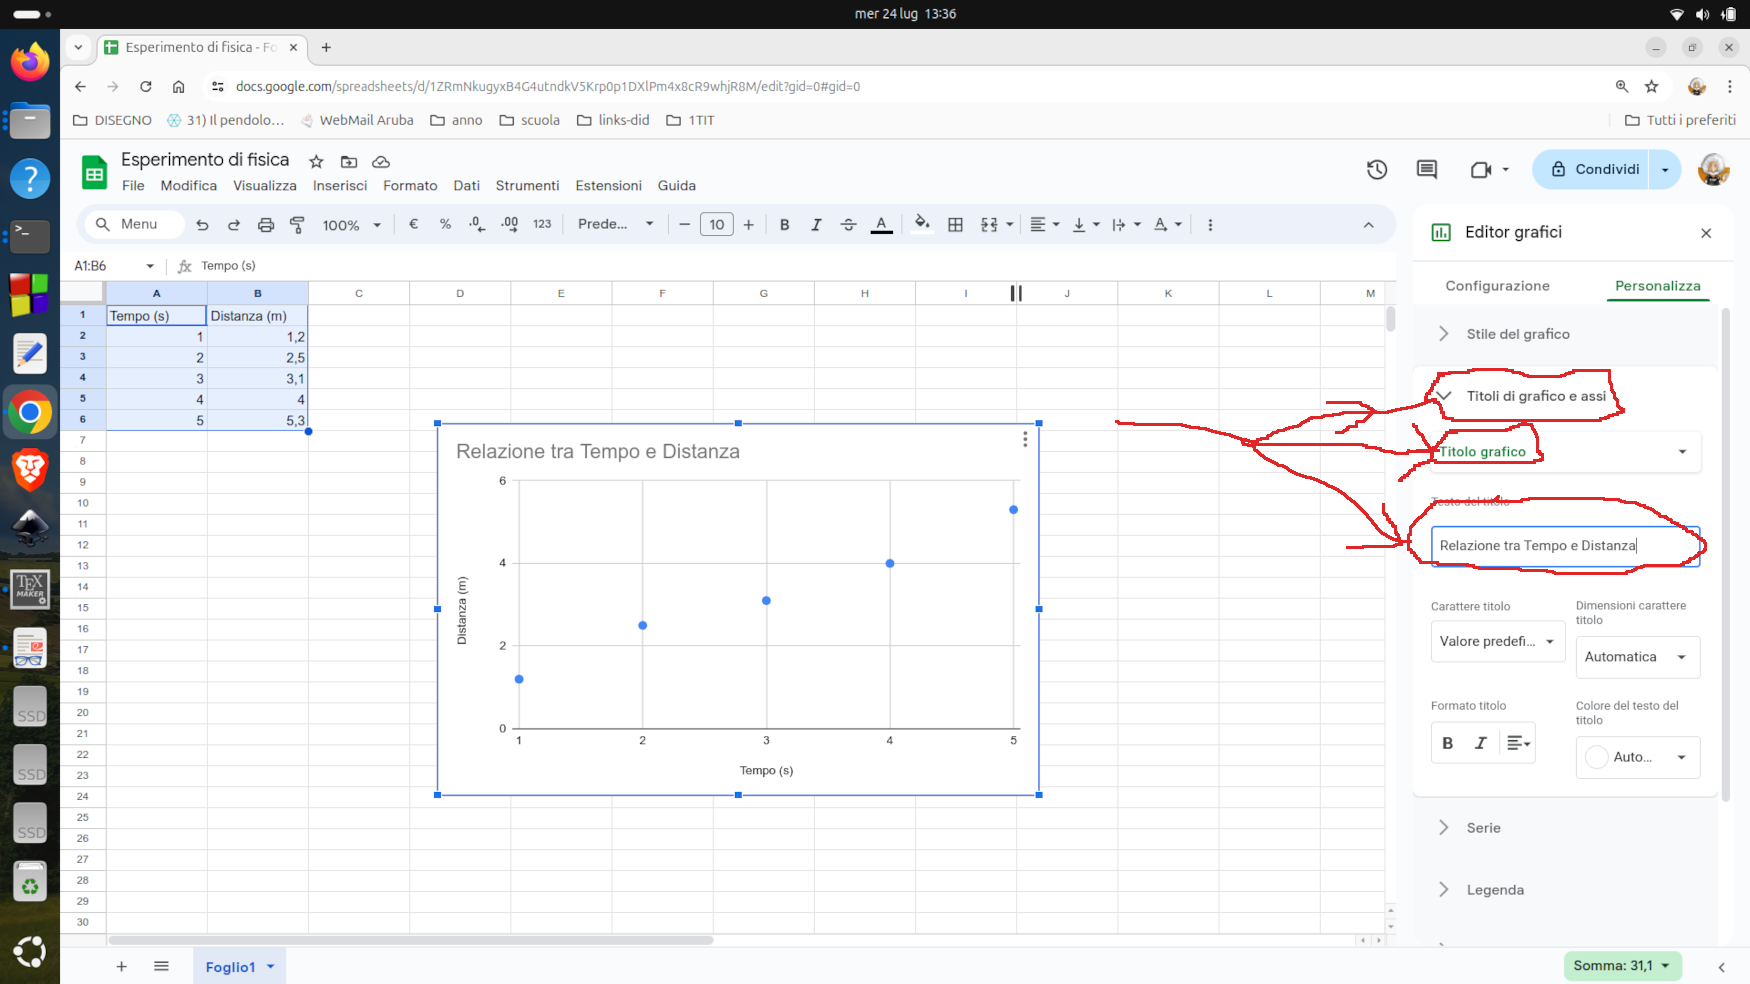
\includegraphics[width=\linewidth]{img/titolo.png} 
    \caption{Scheda \textbf{Modifica del titolo.}}
    \label{fig:titolo}
\end{figure} 
    
    \item Aggiungi le etichette agli assi. Seleziona dal menu a tendina \textbf{Titolo asse orizzontale: } (figura \ref{fig:sceltax})
        \begin{figure}[h!]
    \centering
    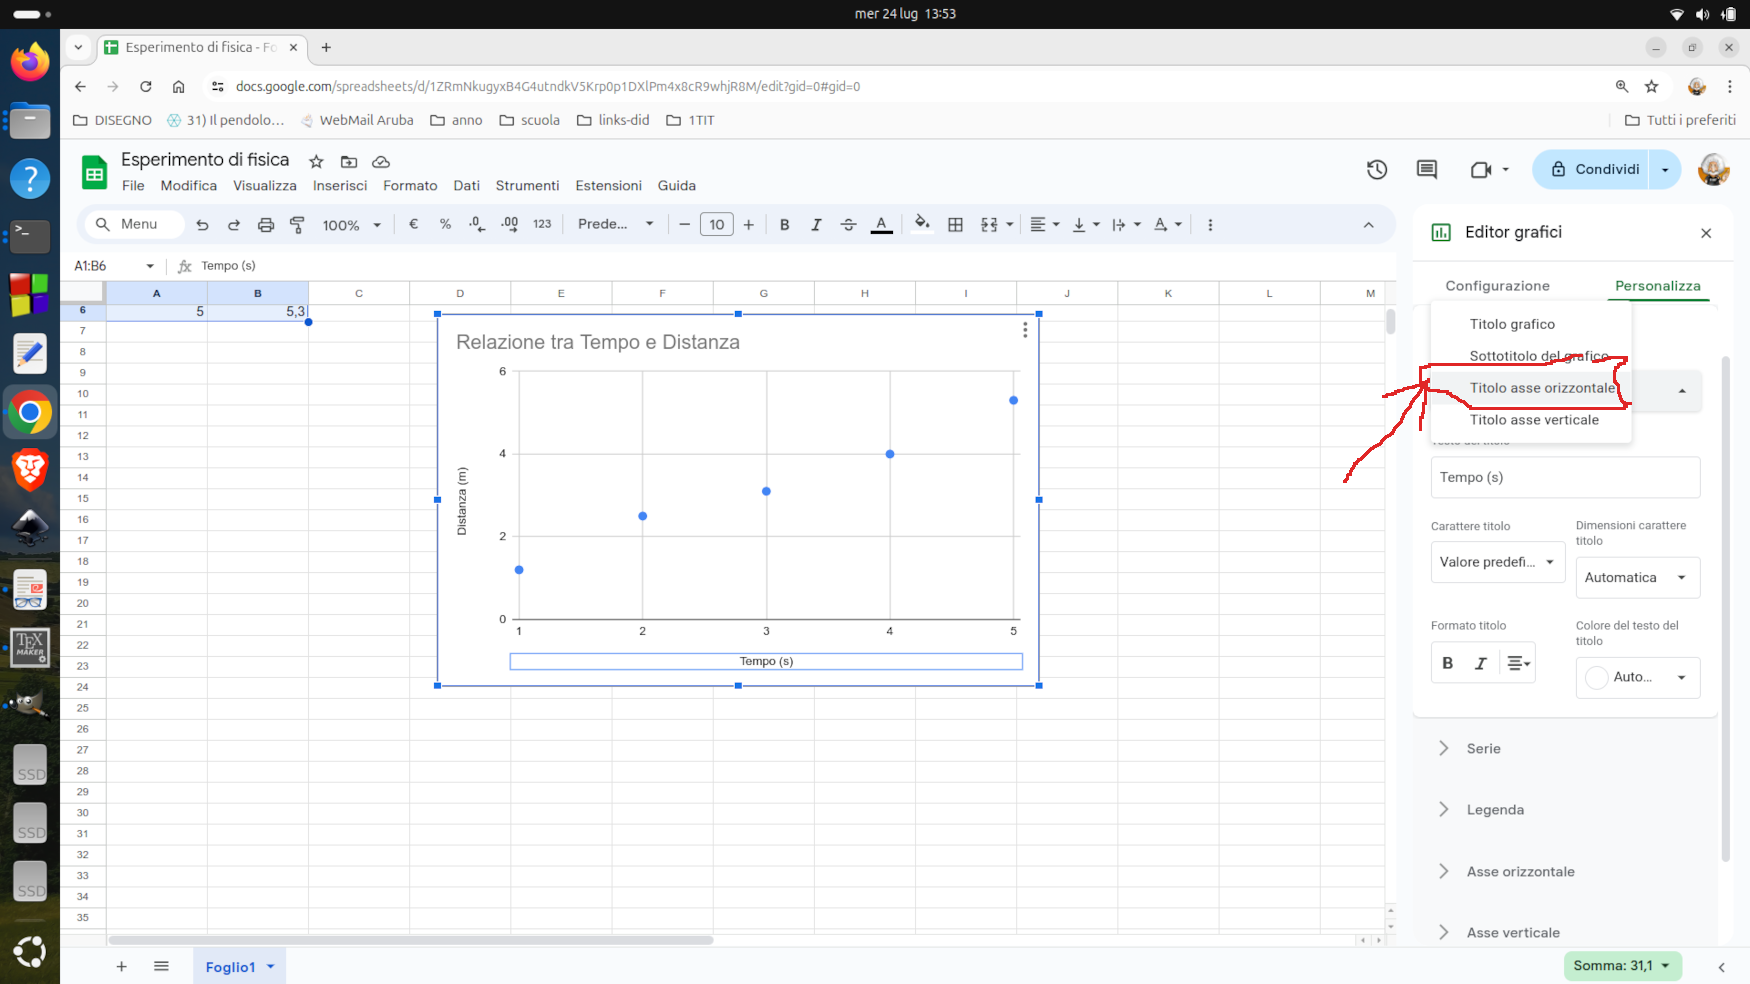
\includegraphics[width=\linewidth]{img/sceltax.png} 
    \caption{Scelta menu per il titolo dell'asse orizzontale.}
    \label{fig:sceltax}
\end{figure}  
        
        
        \item Imposta il titolo per l'asse X: \textit{Tempo (s)} (figura \ref{fig:titolox})
        
       \begin{figure}[h!]
    \centering
    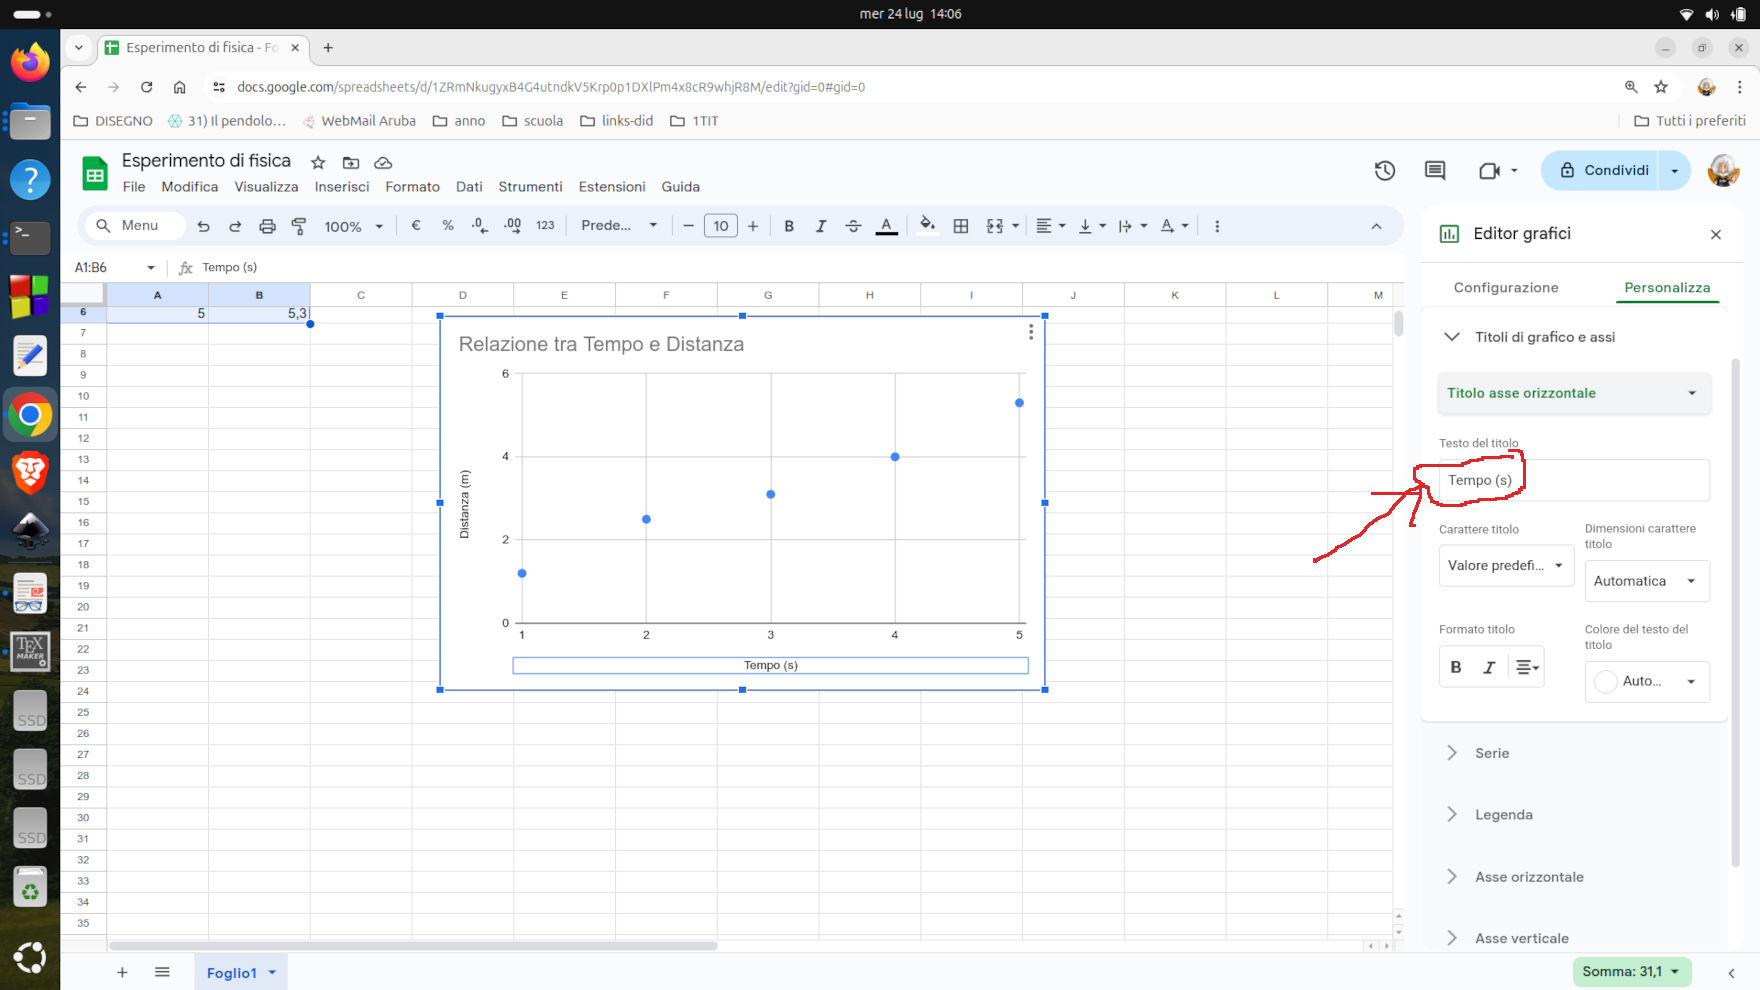
\includegraphics[width=\linewidth]{img/titolox.png} 
    \caption{Scelta del titolo per l'asse x}
    \label{fig:titolox}
\end{figure} 



    \item Seleziona dal menu a tendina \textbf{Titolo asse verticale: } (figura \ref{fig:sceltay}).  
    \begin{figure}[h!]
    \centering
    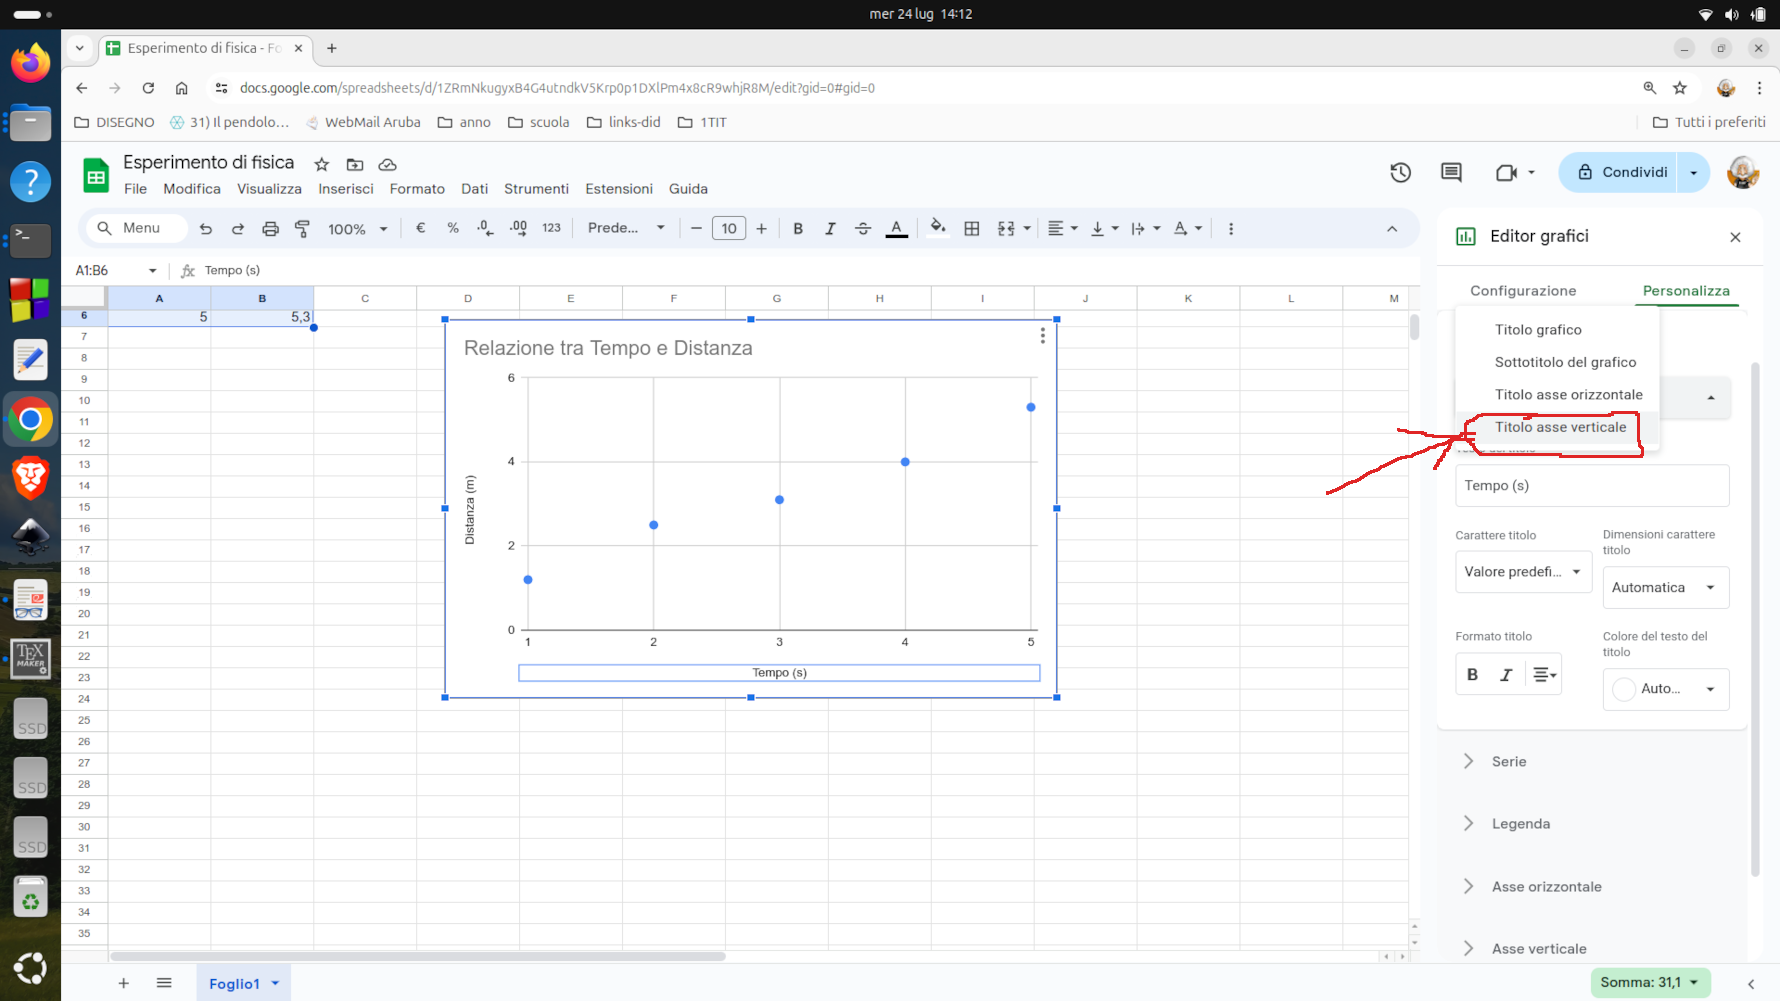
\includegraphics[width=\linewidth]{img/sceltay.png} 
    \caption{Scelta menu per l'asse verticale.}
    \label{fig:sceltay}
\end{figure}  



        \item Imposta un titolo per l'asse  Y: \textit{Distanza (m)} (figura \ref{fig:titoloy})
        
    
\begin{figure}[h!]
    \centering
    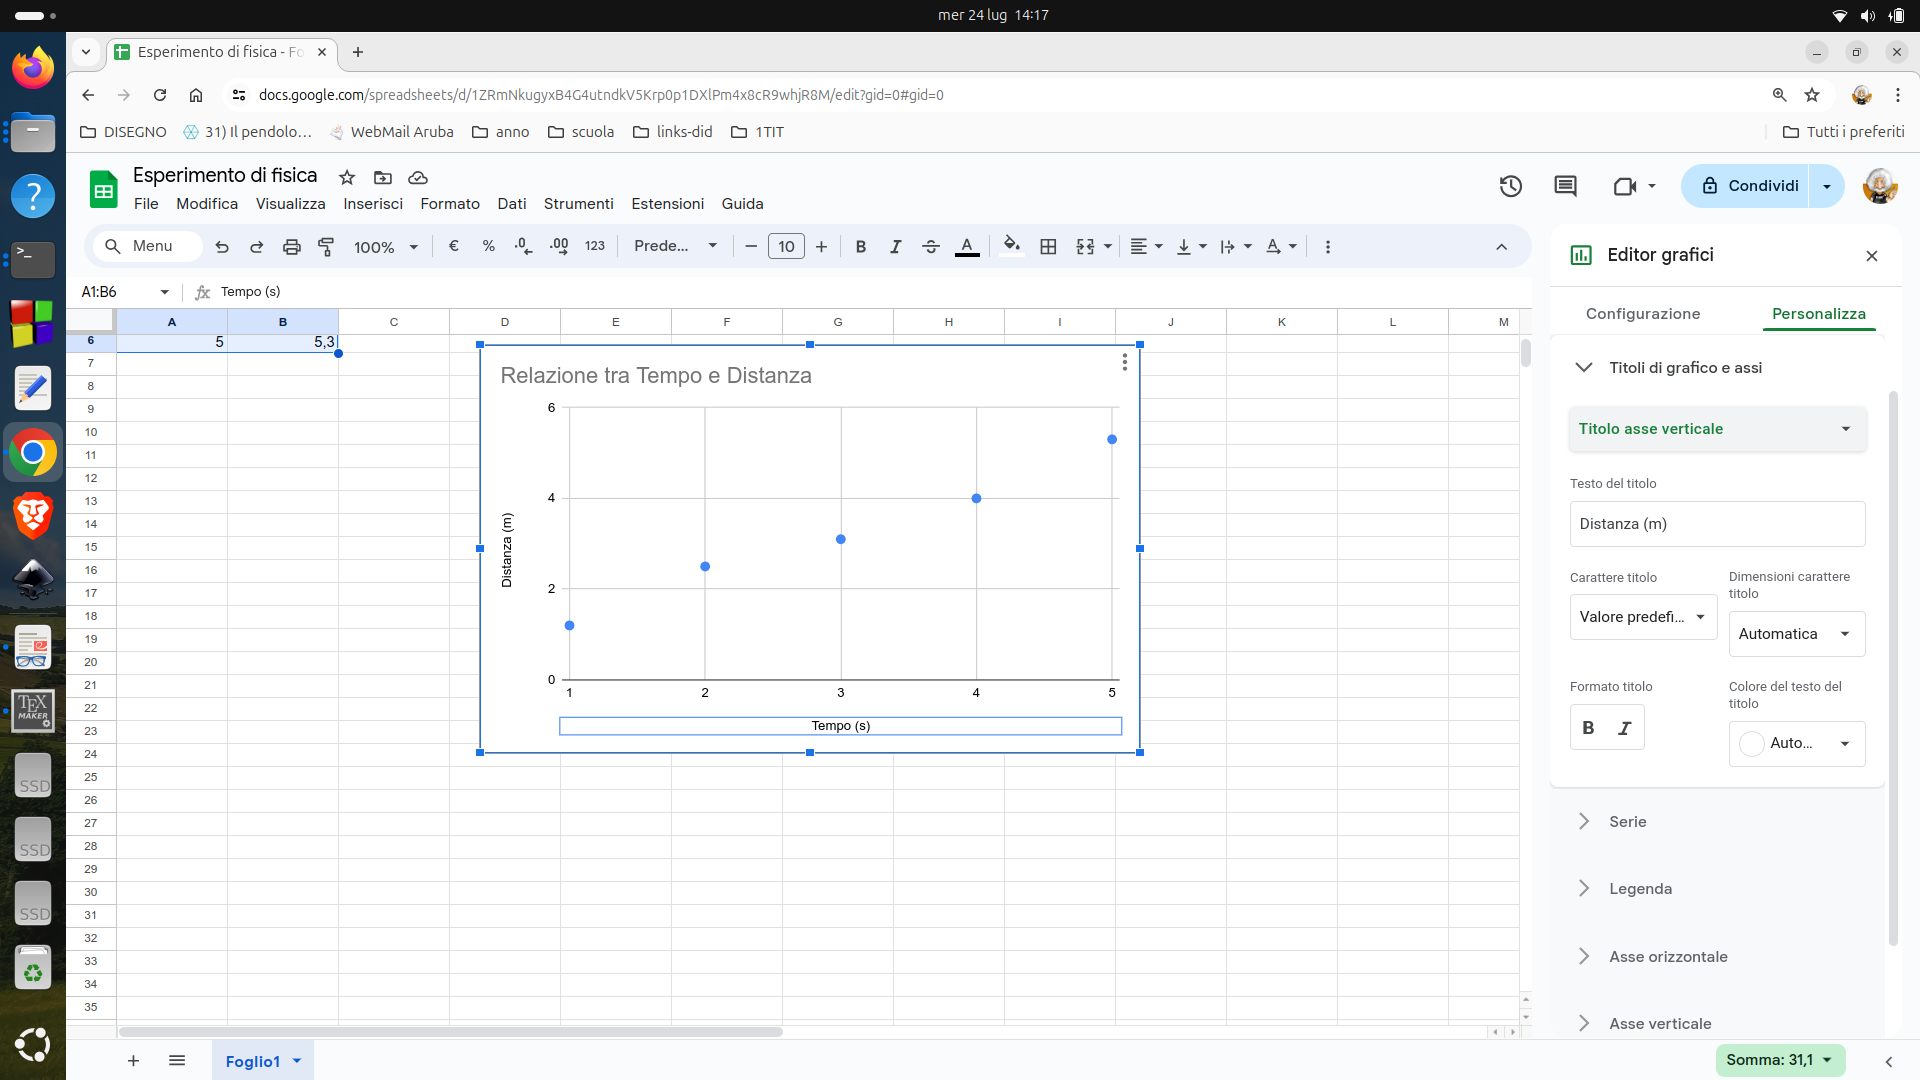
\includegraphics[width=\linewidth]{img/titoloy.png} 
    \caption{Scelta del titolo per l'asse verticale.}
    \label{fig:titoloy}
\end{figure}
        

    \item Per aggiungere una linea di tendenza, espendi il sottomenu \textbf{Serie} (figura \ref{fig:serie}) e seleziona \textbf{Linea di tendenza}. Puoi scegliere il tipo di linea di tendenza (lineare, polinomiale etc.) in base ai tuoi dati. I nostri dati sembrano adattarsi ad una retta, per cui sceglieremo \textbf{Lineare}. In fine. scegliamo di mostrare l'equazione della linea di tendenza (sottomenu \textbf{Etichetta}, voce \textbf{Utilizza equazione}. Si tratta della formula che stiamo cercando, ossia il legame tra X ed Y, figura \ref{fig:tendenza}). Anticipiamo che nel caso specifico, l'equazione mostrata è la formula che lega lo spazio al tempo in un moto rettilineo uniforme. Più avanti la scriveremo nella forma:
    \[
    s=v\cdot t +s_0
    \]
    essendo $s$ la distanza percorsa ad un certo istante $t$, $v$ la velocità costante, ed $s_0$ la posizione iniziale del moto. Possiamo vedere che il corpo si è mosso ad una velocità di $\SI{0,97}{\meter\per\second}$ partendo da una posizione all'istante zero pari a $\SI{0,31}{\meter}$ (figura \ref{fig:polinomiale}). Perché è comoda questa equazione? L'equazione permette di calcolare la posizione ad un qualunque istante, anche se non presente in tabella. Ad esempio, per $t=\SI{2,9}{\second}$, abbiamo:
    
    \[
    s=\left(\SI{0,97}{\meter\per\second}\right)\times \left( \SI{2,9}{\second}\right) + \SI{0,31}{\meter}=\SI{3,12}{\meter}.
    \]
    
\begin{figure}[h!]
    \centering
    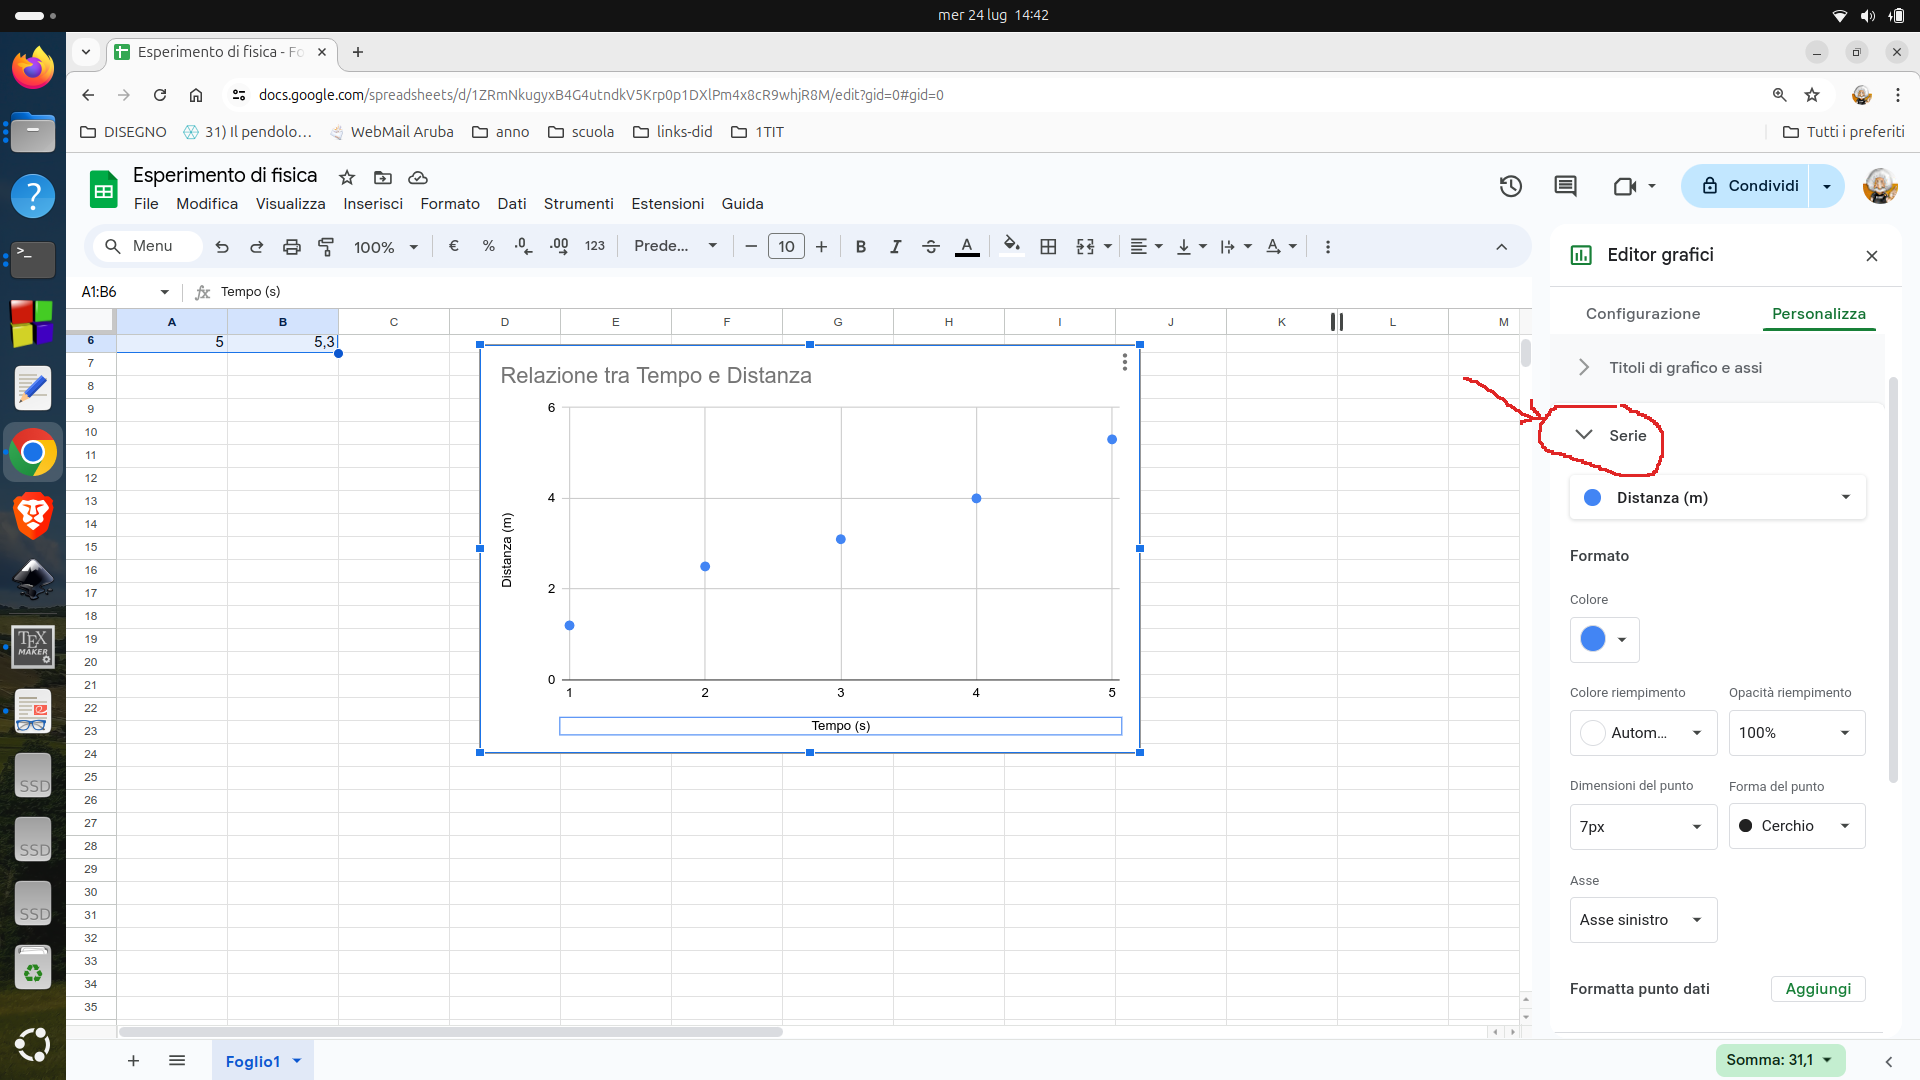
\includegraphics[width=\linewidth]{img/serie.png} 
    \caption{Scheda \textbf{serie} per la linea di tendenza.}
    \label{fig:serie}
\end{figure}    
  \begin{figure}[h!]
    \centering
    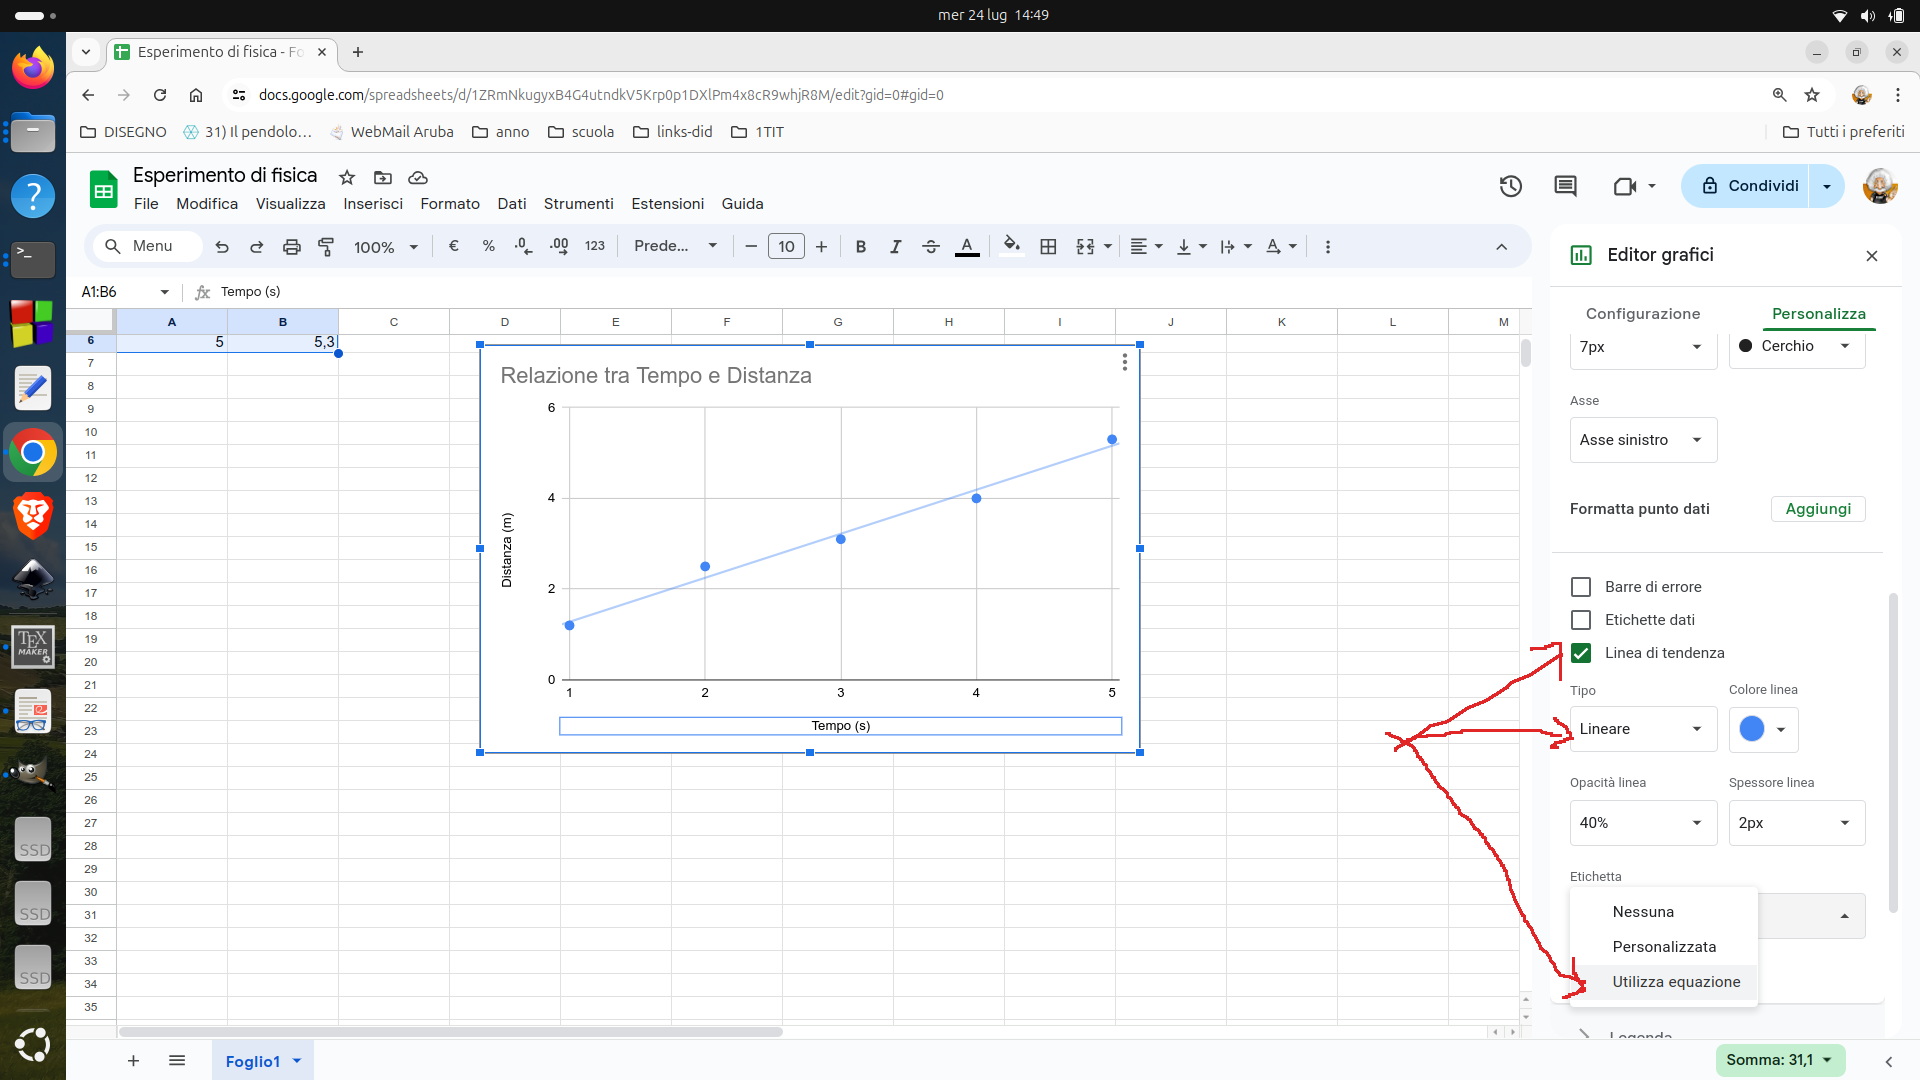
\includegraphics[width=\linewidth]{img/tendenza.png} 
    \caption{Scheda \textbf{serie} Inserimento linea di tendenza lineare (retta).}
    \label{fig:tendenza}
\end{figure}    
   In generale non è facile scegliere il tipo di linea di tendenza. In fisica, i dati possono essere legati da una relazione di proporzionalità diretta, quadratica, inversa, quadratica inversa o molte altre. Il tipo lineare è il più semplice. Quando i grafici hanno un andamento curvo, è possibile che i dati siano legati da una formula parabolica (ossia una formula del tipo $y=ax^2 +bx +c$.) In questo caso, la linea di tendenza sarà una parabola. Nei fogli google, basterà selezionare dal sottomenu la linea \textbf{Polinomiale} (figura \ref{fig:polinomiale}):
   \begin{figure}[h!]
    \centering
    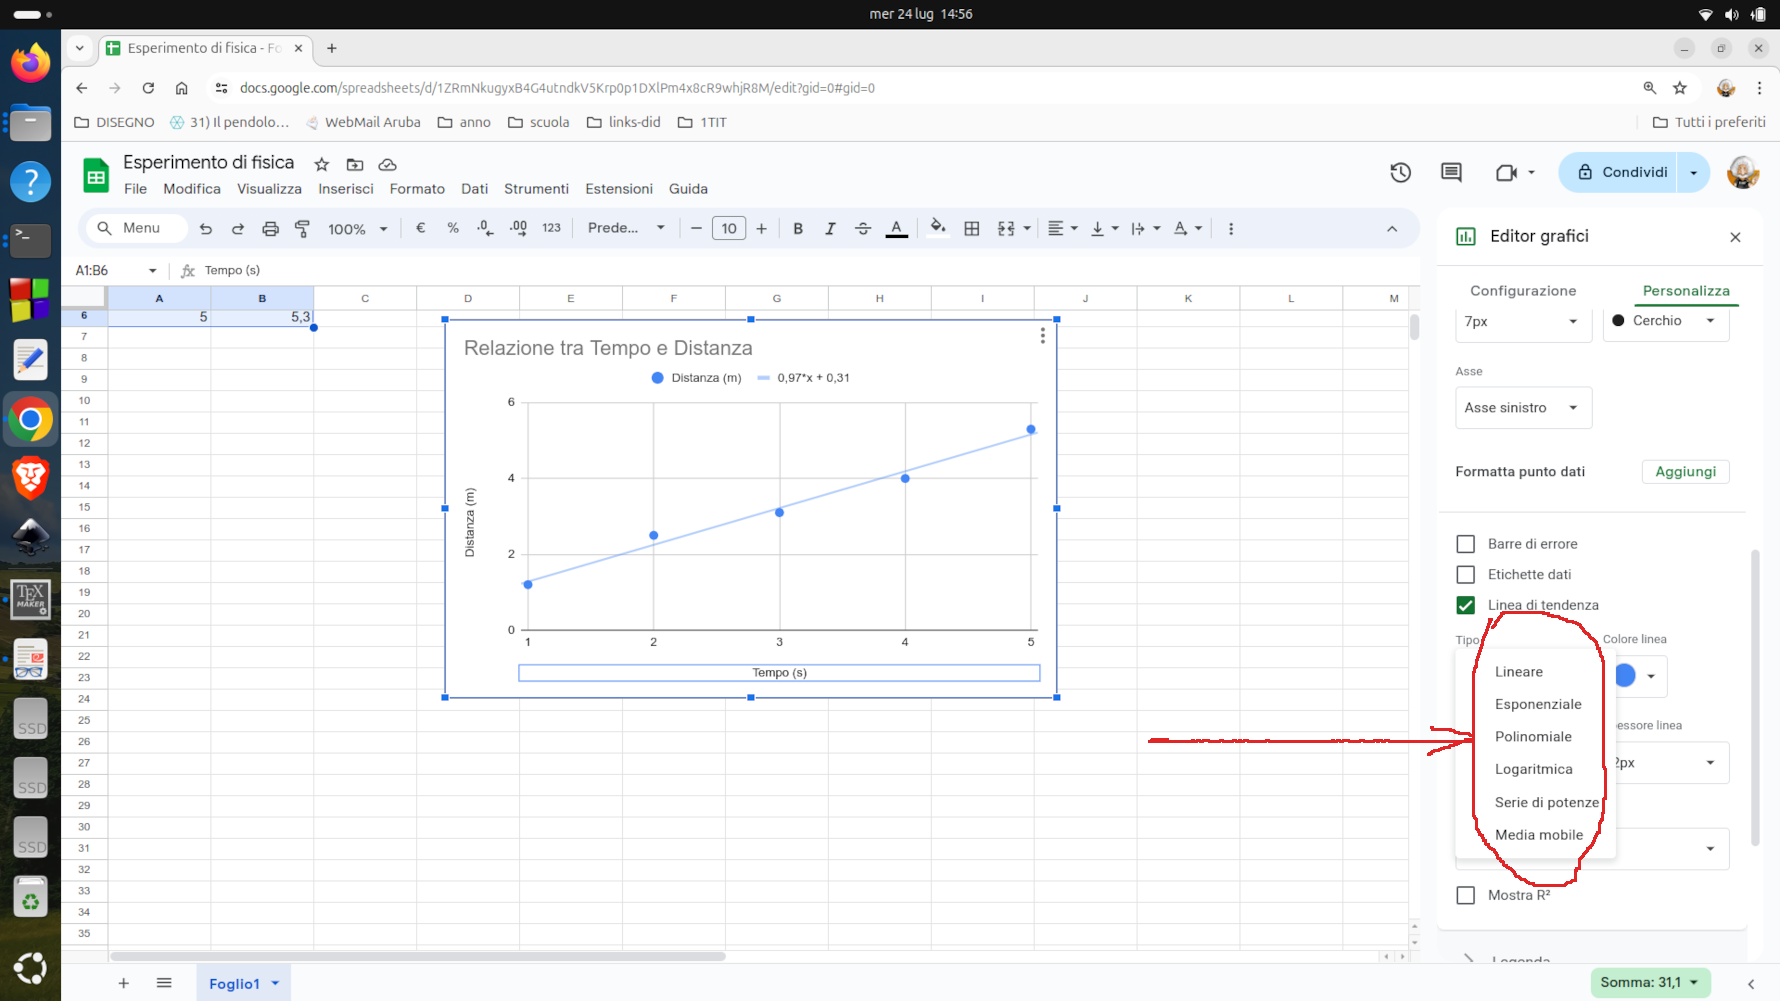
\includegraphics[width=\linewidth]{img/polinomiale.png} 
    \caption{Scelta per l'inserimento della linea di tendenza polinomiale (parabola).}
    \label{fig:polinomiale}
\end{figure}     
 In generale, ti consiglio di provare varie linee di tendenza, in modo da trovare quella che meglio si adatta ai dati.    L'adattamento è tanto migliore quanto più il cosiddetto fatto $R^2$ è vicino ad uno. Per visualizzare questo fattore sul grafico, barrare la casella $\mathbf{Mostra \,\,R^2}$ come in figura \ref{fig:r2}:
 
   \begin{figure}[h!]
    \centering
    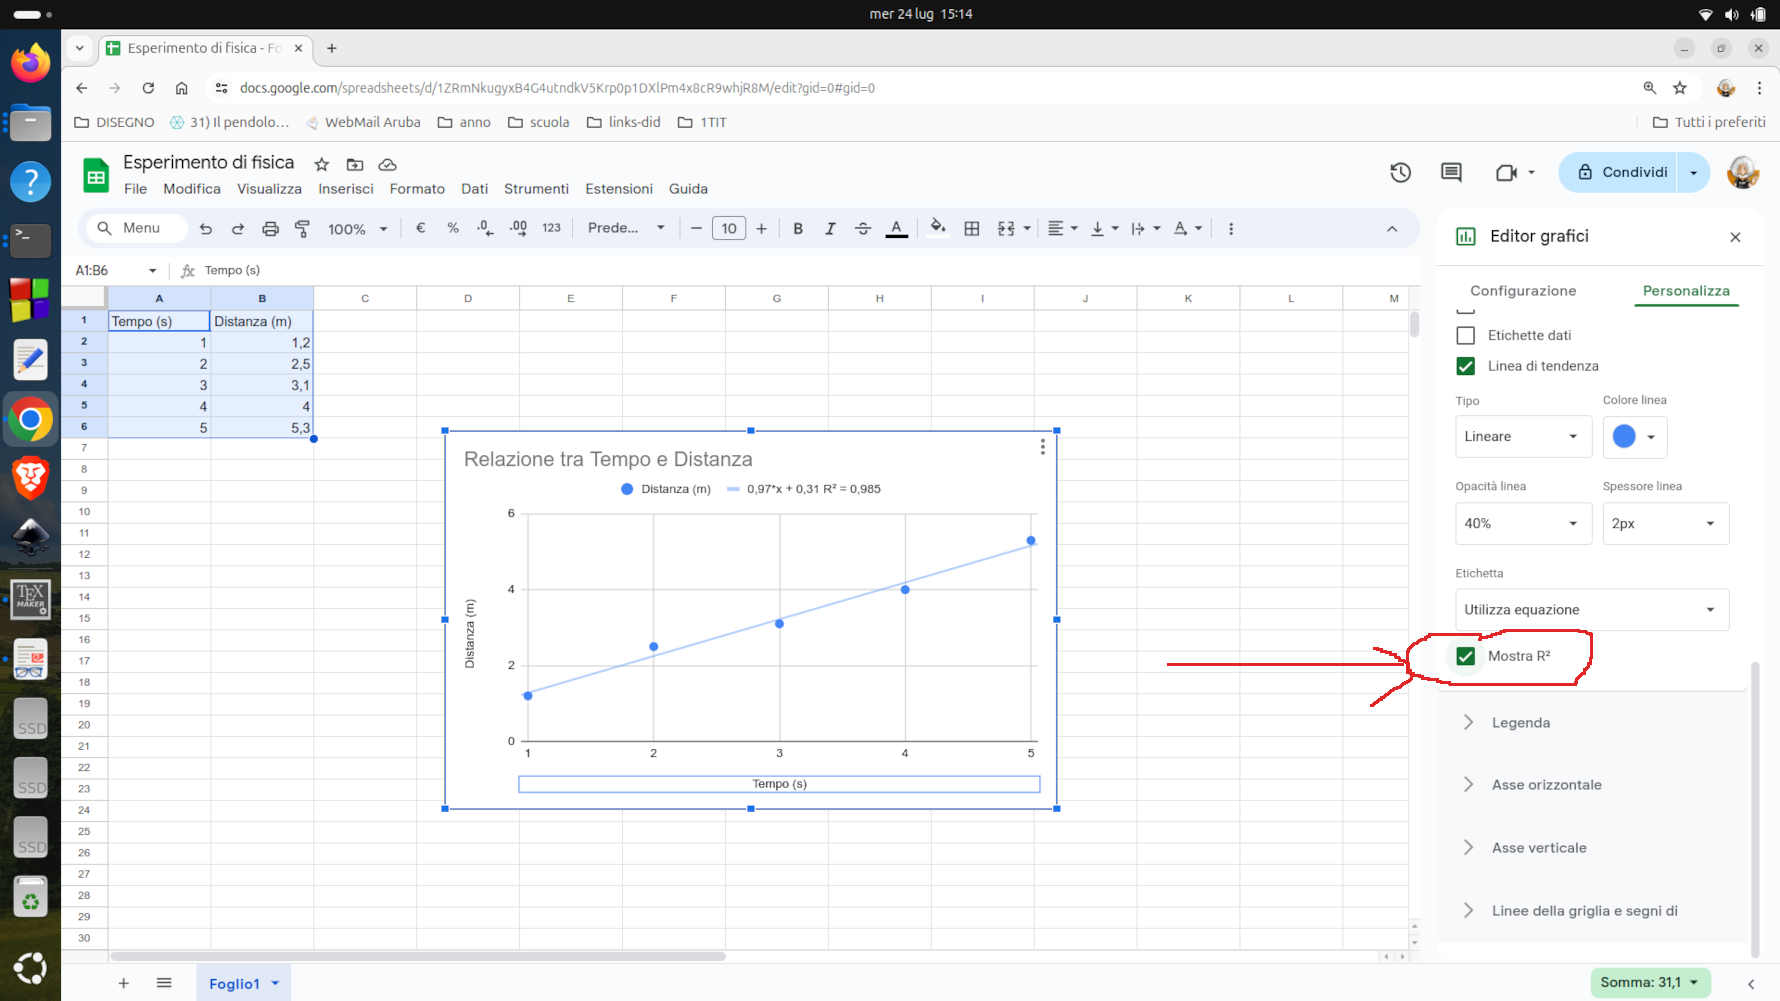
\includegraphics[width=\linewidth]{img/r2.png} 
    \caption{Visualizzazione del parametro $R^2$.}
    \label{fig:r2}
 \end{figure}
 
    
\end{enumerate}
Tutti gli elementi grafici e  testuali sono ulteriormente personalizzabili (ad esempio l'aspetto dei punti del grafico, il font per i titoli degli assi etc.). Ti consiglio di sperimentare con questi aspetti modificando a tuo piacimento questi elementi dalla scheda personalizzazione. Il loro uso è molto intuitivo.

\subsection{Visualizzare due Grafici Contemporaneamente}
\begin{enumerate}
    \item Inserisci una nuova serie di dati in una colonna diversa. Ad esempio, nella colonna C metti i valori della variabile dipendente di un secondo esperimento (ad esempio, distanza in metri).
    \item Esempio di dati:
    \begin{center}
    \begin{tabular}{|c|c|c|}
    \hline
    Tempo (s) & Distanza 1 (m) & Distanza 2 (m) \\
    \hline
    1 & 1,2 & 0,8 \\
    2 & 2,5 & 1,5 \\
    3 & 3,1 & 2,2 \\
    4 & 4,0 & 3,0 \\
    5 & 5,3 & 4,1 \\
    \hline
    \end{tabular}
    \end{center}
    \item Seleziona i dati inseriti nelle colonne A, B e C. Puoi farlo cliccando e trascinando il mouse dall'angolo superiore sinistro (A1) all'angolo inferiore destro (C5) dei tuoi dati oppure (vedi figura \ref{fig:intervallo2}) selezionando \textbf{aggiungi serie}, figura \ref{fig:intervallo2} e. successivamente, cliccando il tasto ``+''. Si aprirà un campo di testo in cui inserire l'intervallo di cella. Per farlo, si può agire graficamente, selezionando tutta la colonna col tasto destro del mouse e verrà automaticamente scritto l'intervallo (figura \ref{fig:intervallo2-dialogo}. La scrittura \textit{Foglio1!C1:C6} indica di selezionare l'intervallo del foglio attuale (Foglio1) dalla cella C1 alla cella C6). In fine clicca ``Ok'' e la serie verrà inserita. A questo punto puoi personalizzare il grafico come vuoi, inserire linee di tendenza etc. Come regola generale, si consiglia di realizzare grafici in cui le due serie sullì'asse Y sono della stessa natura ma non è vietato inserire anche serie diverse purché, è bene ribadirlo, sull'asse X, ci sia una sola serie per entrambe le grandezze dipendenti (ossia le Y, nel nostro caso, il tempo). Come esercizio, puoi provare a disegnare la linea di tendenza della serie 2. Il grafico finale è in figura \ref{fig:finale}.
    
      \begin{figure}[h!]
    \centering
    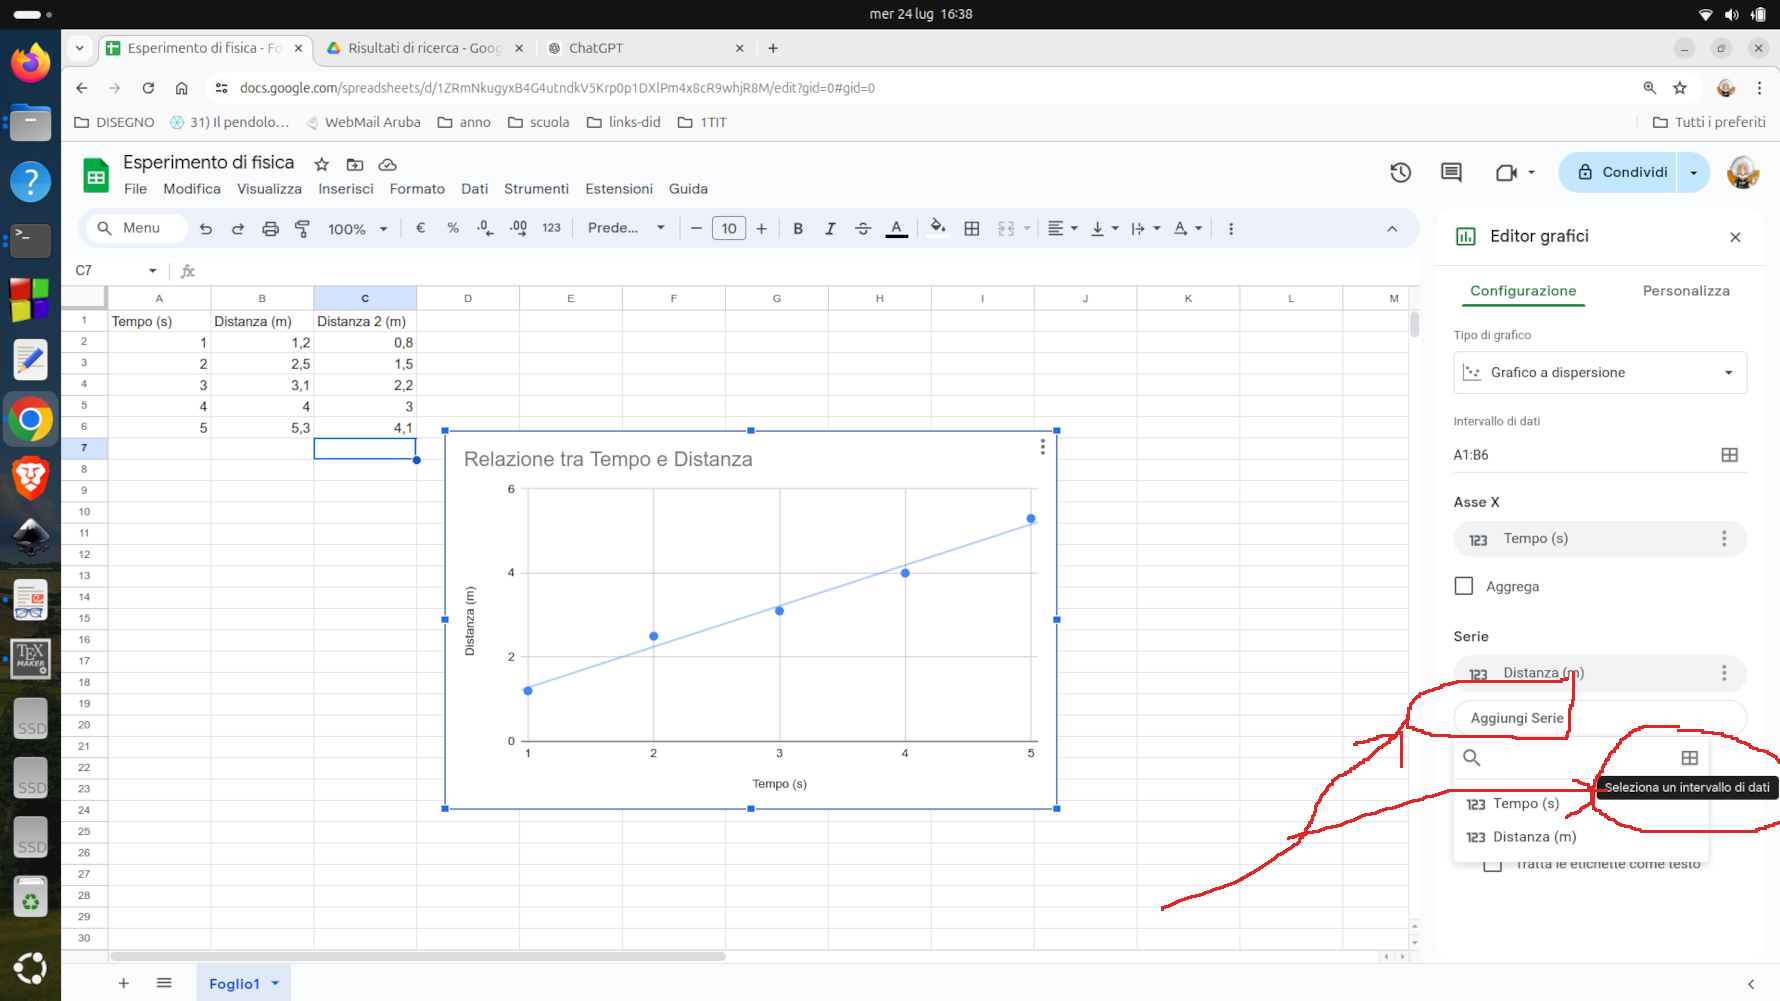
\includegraphics[width=\linewidth]{img/intervallo2.png} 
    \caption{Selezione di una serie, tasto ``+''.}
    \label{fig:intervallo2}
 \end{figure} 
    
    
\begin{figure}[h!]
    \centering
    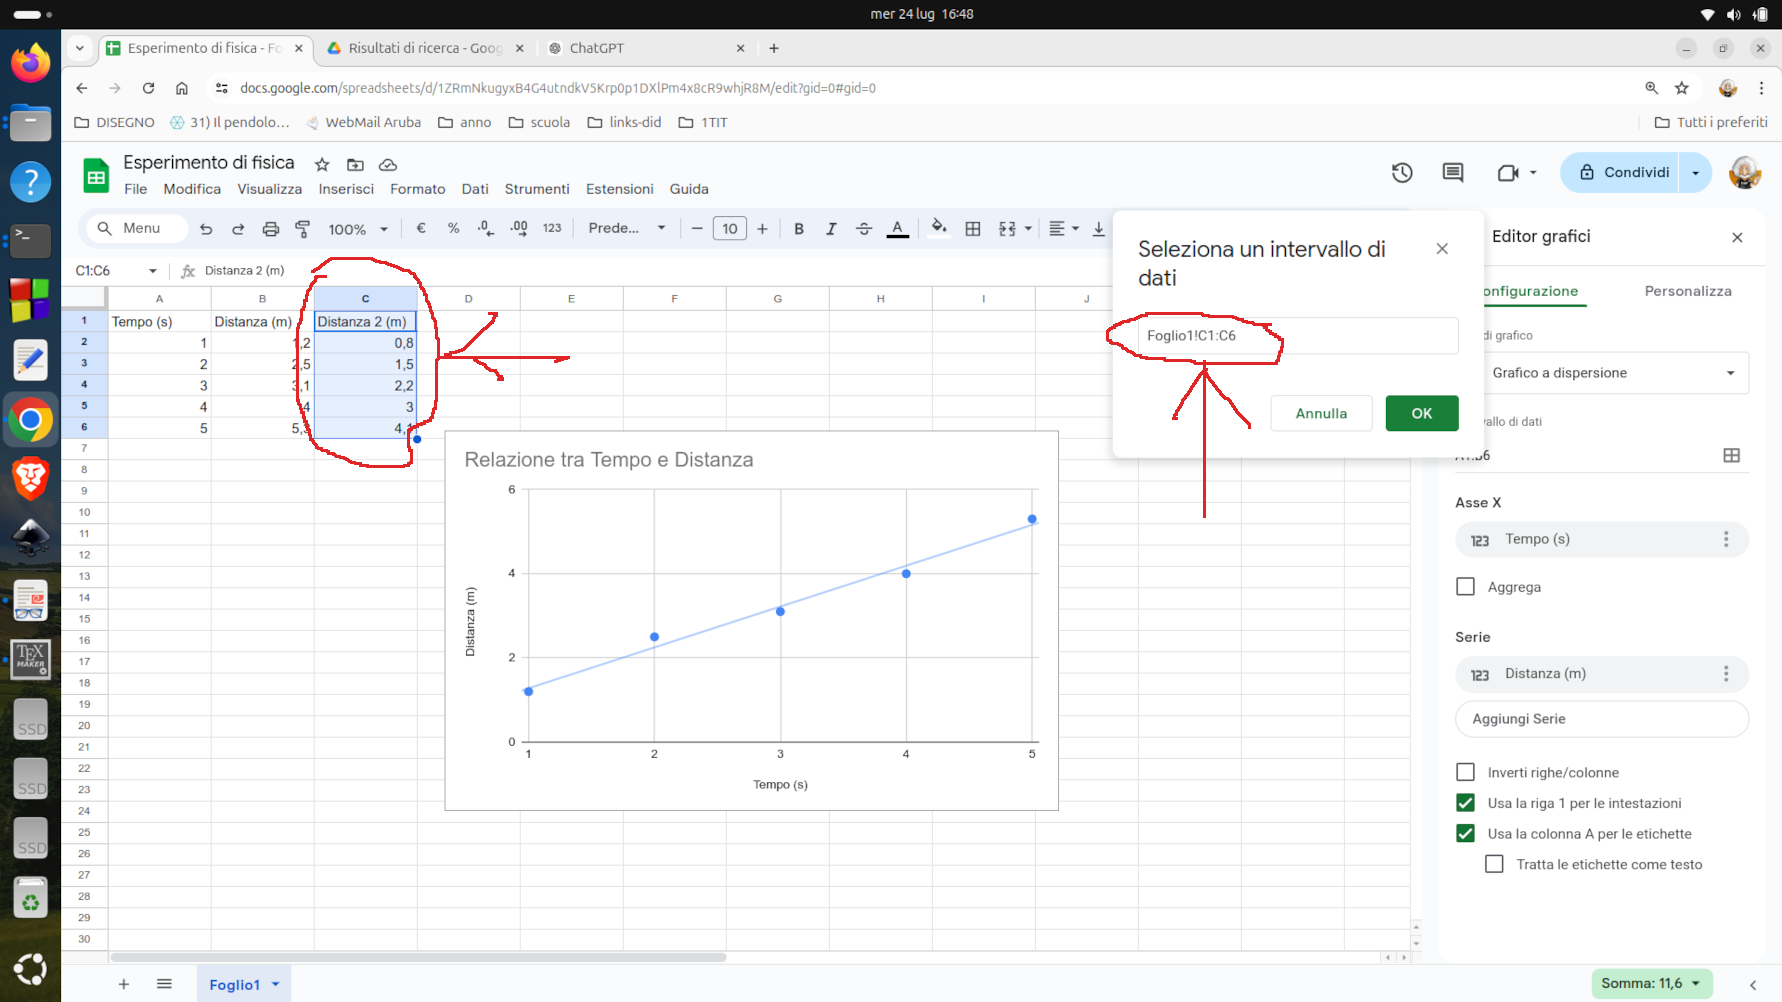
\includegraphics[width=\linewidth]{img/intervallo2-dialogo.png} 
    \caption{Finestra di dialogo per la scelta dell'intervallo della serie 2.}
    \label{fig:intervallo2-dialogo}
 \end{figure} 

\begin{figure}[h!]
    \centering
    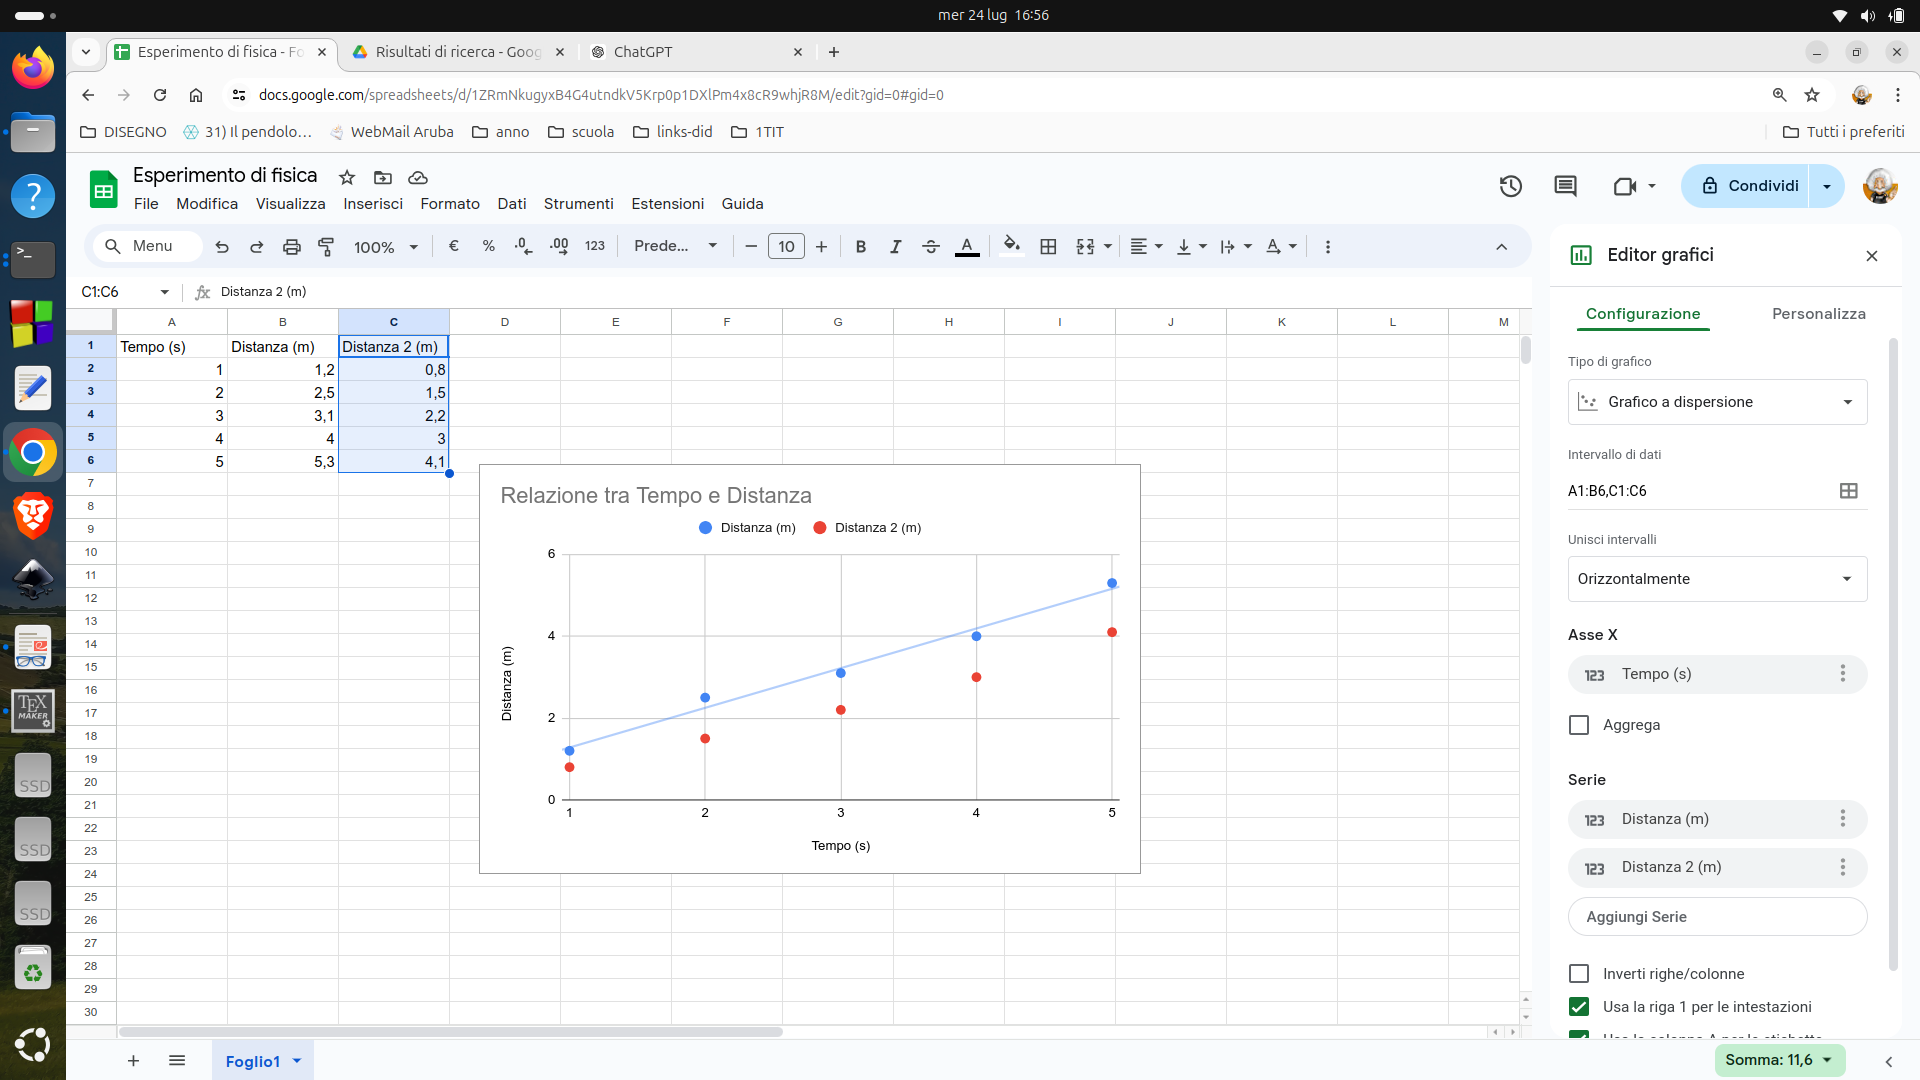
\includegraphics[width=\linewidth]{img/finale.png} 
    \caption{Come si presenta il grafico costruito nel tutorial.}
    \label{fig:finale}
 \end{figure} 
\end{enumerate}





\subsection{Conclusione}
Seguendo questi passaggi, sarai in grado di creare e personalizzare grafici a dispersione su Google Sheets per analizzare e visualizzare i tuoi dati sperimentali. Questa competenza è utile non solo per le lezioni di fisica, ma anche per altre discipline scientifiche.

